\documentclass[a4paper,11pt]{report}
%DRAFT: remove this option to disable all teacher notes.

\usepackage{amsmath}
\usepackage{amssymb}

\usepackage[obeyDraft]{todonotes}

\newcommand{\question}[1]{\todo[color=green!40,inline]{\textbf{Question}: #1}}
\newcommand{\comment}[1]{\todo[color=white,inline]{#1}}


\usepackage{amsthm}

\theoremstyle{definition}
\newtheorem{definition}{Definition}
\theoremstyle{remark}
\newtheorem{note}{Note}

\theoremstyle{plain}
\newtheorem{example}{Example}
\newtheorem{lem}{Lemma}




\begin{document}
	\title{DAT650 Blockchain Technology - Course Script}
	\author{Leander Jehl}
	\date{\today}
	
	\maketitle

\chapter{Data structures}
\label{ch:hashchain}

%!TEX root = ../main.tex

\section{Hash Function}
\comment{Repetition from DAT510}

\question{Do you remember what a hash function is?}
\question{What is the most common use case for not cryptographic a hash function?}

\begin{definition}
	A (cryptographic) \textbf{hash function} $H$ $(H(x) \mapsto y)$ is a \emph{deterministic} function that maps inputs ($x$) of arbitrary size to "small" outputs ($y$), e.g. 256 bit numbers.
\end{definition}
 
\begin{note}
The idea for a hash function is that the result should "look" random. 
However the function is \emph{deterministic}, i.e. the same input always results in the same output.
\end{note}

\begin{note}
A mental image for a hash function is the following:

Imagine a gnome that lives in a closed box. When you give a new peace of text to the gnome, he writes down the text, roles some dice and gives you a random number for your text.

When given the next peace of text, the gnome will look up if he has seen this text before. If yes, he will return the number from before. If no, he roles the dice and gives you a new number.
\end{note}
\question{Do there exist two $x$ that have the same hash value?}
\question{Assume hashes are 4-bits. Can you find a string or text that has the hash value? How long will it take?}

\begin{example}
Example for hash functions are

\begin{description}
	\item[MD5] not secure
	\item[SHA-1] not secure
	\item[SHA-2] actually SHA-256 and SHA-512 give 256 and 512 bit output.
	\item[SHA-3] standard from 2015
\end{description}

On unix terminal (also mac) compute SHA-256 of a file
\begin{verbatim}
shasum -a 256 file.txt	
\end{verbatim}
or
\begin{verbatim}
	printf "hello world" | shasum -a 256
\end{verbatim}
Hashes here are given in hexadecimal numbers.
\end{example}


\question{With hexadecimal numbers, how many characters are needed to represent a 64 bit hash?}
\comment{ use echo -n "hash" 
(pipe) wc -c	
 to count characters = 64}



\begin{definition}
	For a secure hash function the following security properties need to hold:
	\begin{description}
		\item[Pre-image resistance] (one way) Given a d-bit $y$ it is infeasible to find any $x$ such that $y= H(x)$
		\item[Weak collision resistance] Given an input $x$ it is infeasible to find a different $x'$ such that $H(x) = H(x')$.
		\item[Collision resistance] It is infeasible to find inputs $x$ and $x'$
		such that $x \neq x'$ and $H(x)=H(x')$.
	\end{description}
	\emph{Infeasibility} means that an exhaustive search is the best strategy to find such values and the probability to find an $x$ as above is smaller than $\frac{1}{2^{112}}$
\end{definition}

\question{Which property is hardest to get? -> Birthday paradox with dice.}
\question{Think of examples how to use a cryptographic secure hash function?}

\begin{example}
Examples for the use of cryptographic hash functions are:
\begin{itemize}
	\item Including hashes of third party content in HTML-tags, e.g. scripts.
	\item Not storing user passwords in plain text.
\end{itemize}
\end{example}

\question{Given a secure hash functions, how can we define a large number of secure hash functions and randomly select one of them? E.g. a different hash function for every user of a website.}

\begin{note}
Given a secure hash function $H$ that takes strings as input, we can create a hash function $H'$ that takes lists, structs or byte arrays as input.

For pre-image resistance to be useful, the domain of structs should be large and structs should be unpredictable.
\end{note}

\comment{English has about 150 000 words in use. Random 4 letter combinations are more than 400 000.}


\begin{note}
Given a hash function $H: \mathcal{X} \rightarrow \mathcal{Y}$ that hashes strings (or byte slices) we can create a hash function $H: \mathcal{X} \times \mathcal{X} \rightarrow \mathcal{Y}$ by concatenating the inputs.

We write $x_1|| x_2$ for the concatenation of inputs $x_1$ and $x_2$.
Note that the resulting hash function is not commutative.
\[
H(x_1||x_2) \neq H(x_2|| x_1)
\]
\end{note}

%!TEX root = ../main.tex

\section{Hash chain}

Assume that $H$ is a secure hash function that maps a struct to a 256-bit.

\begin{definition}
A \textbf{hash-chain} is a data-structure composed of nodes called blocks. 
Every block $b$ contains a pointer $b.prev$ to a preceding bock and a field $b.h_{-1}$ 
that contains the hash of the block referenced by $b.prev$.
A block also contains a data item $b.data$.

\begin{itemize}
	\item The hash of a block $b$ is computed as $H(b)= H(b.h_{-1} || b.data)$.
	\item $b.h_{-1}=H(b.prev)$
	\item There exist one block $b_0$, for which $b.prev$ is empty.
	\item For to block $b$ and $b'$, if $b.prev=b'$ we say that $b$ is a \emph{successor} of $b'$.
	
\end{itemize}

In a \textbf{hash-chain} every block has at most one successor.
\end{definition}


\comment{Image}

\begin{lem}
The blocks in a hash-chain can be linearly ordered according to the successor relation with the block $b_0$ as the first block.
\end{lem}


\begin{note}
	If blocks $b_0$, $b_1$ and $b_2$ contain data $D_0$, $D_1$ and $D_2$ then
\begin{align*}
	H(b_0) & = H(D_0)\\
	H(b_1) & = H( H(b_0) || D_1) = H( H(D_0)|| D_1) \\
	H(b_2) & = H( H(b_1) || D_2) = H( H(D_0)|| D_1) \\
\end{align*}

\end{note}


\question{Given a hash chain $b_0, b_1, b_2, ..., b_n$ which of the following is infeasible.
\begin{itemize}
	\item Create an alternative hash chain $b'_0, b_1, b'_2, ... ,b'_n$ 
	such that $b'_i=b_i$ for $i<3$ and $b'_3 \neq b_3$.
	\item Create an alternative hash chain $b'_0, b_1, b'_2, ... ,b'_n$ such that $b'_n=b_n$ and $b'_1 \neq b_1$.
	\item Create an alternative hash chain $b'_0, b_1, b'_2$ such that $b'_2=b_1$.
	\item Create an alternative hash chain $b'_0, b_1, b'_2, ... ,b'_n, b'_{n+1}$ such that $b'_{n+1}=b_n$.
	\item Assume $n$ is very large, but no $b_i$ has $b_i.data = "hello world"$.
	Create $b'$, s.t., for some $i\leq n$ $H(b')=H(b_i)$ and $b'.data="hello world"$
\end{itemize}
Why?}

\begin{example}
Assume a notary maintains, a hash-chain of all documents it has signed. 
\begin{itemize}
	\item This allows document holders to proof that their document was signed.
	\item This allows to document holders to proof which document was signed first.
	\item Prevent the notary itself to change in which order documents where signed or remove single documents.
\end{itemize}
\end{example}
\question{How can we publish this hash chain?}
\question{What if the notary has very many documents. Can we avoid to have only one document per block? 
Ideas:
\begin{itemize}
	\item Publish multiple hashes?
	\item Hash multiple documents?
\end{itemize}}

%!TEX root = ../main.tex

\section{Merkle trees}
By publishing a hash of a document/data we can commit to this document, without revealing it. In the following we look at how to publish many such hashes concurrently.

\begin{example}
Given a document describing an invention, I can publish the hash of the document in a newspaper. If someone else then tries to claim my invention, I can proof that I had the document before the date in the newspaper.

This does not reveal my invention.
\end{example}

\begin{example}
In a election you can hash your vote and publish the hash of your vote. After some deadline, you can then reveal your vote to be counted.

\textbf{Problem:} An adversary can simply hash all possible values to vote for and thus discover your vote.

\textbf{Solution:} Hash vote, concatenated with random value.
\end{example}

\subsection{Committing to multiple values}
Given data $D_1$, $D_2$, $D_3$ and $D_4$. We want to commit to all four values.
We can either publish individual hashes or a single hash for all:
\begin{enumerate}[label=\alph*)]
	\item Publish $[H(D_1),H(D_2),H(D_3),H(D_4)]$.
	\item Publish $H(D_1||D_2||D_3||D_4)$.
\end{enumerate}

Variant b) requires to publish only a single hash. However to proof that $D_1$ was committed to, it is necessary to reveal also $D_2$, $D_3$, and $D_4$.

\begin{example}
We can build on scheme a) and additionally create $h_{1,2}=H(H(D_1) || H(D_2))$, 
$h_{3,4} H(H(D_3) || H(D_4))$ and $h_{1,2,3,4}= H(h_{1,2}|| h_{3,4})$.

We publish $h_{1,2,3,4}$. 

To prove that $D_3$ was included we present $D_3$, $h_4=H(D_4)$ and $h_{1,2}$.
To check the proof, recompute $h_{3,4}$ and $h_{1,2,3,4}$.
\end{example}

\begin{definition}
	A \textbf{Merkle Tree} is a (binary) tree where every note is labeled with a hash $h$.
	\begin{itemize}
		\item For internal nodes $h$ is the hash of the concatenated labels of its children ($h=H(\mathit{leftchild}.h||\mathit{rightchild}.h)$).
		\item For a leaf node, $h$ is the hash of the data stored in the node ($h=H(D_i)$).
	\end{itemize}
\end{definition}

\begin{figure}[ht]
	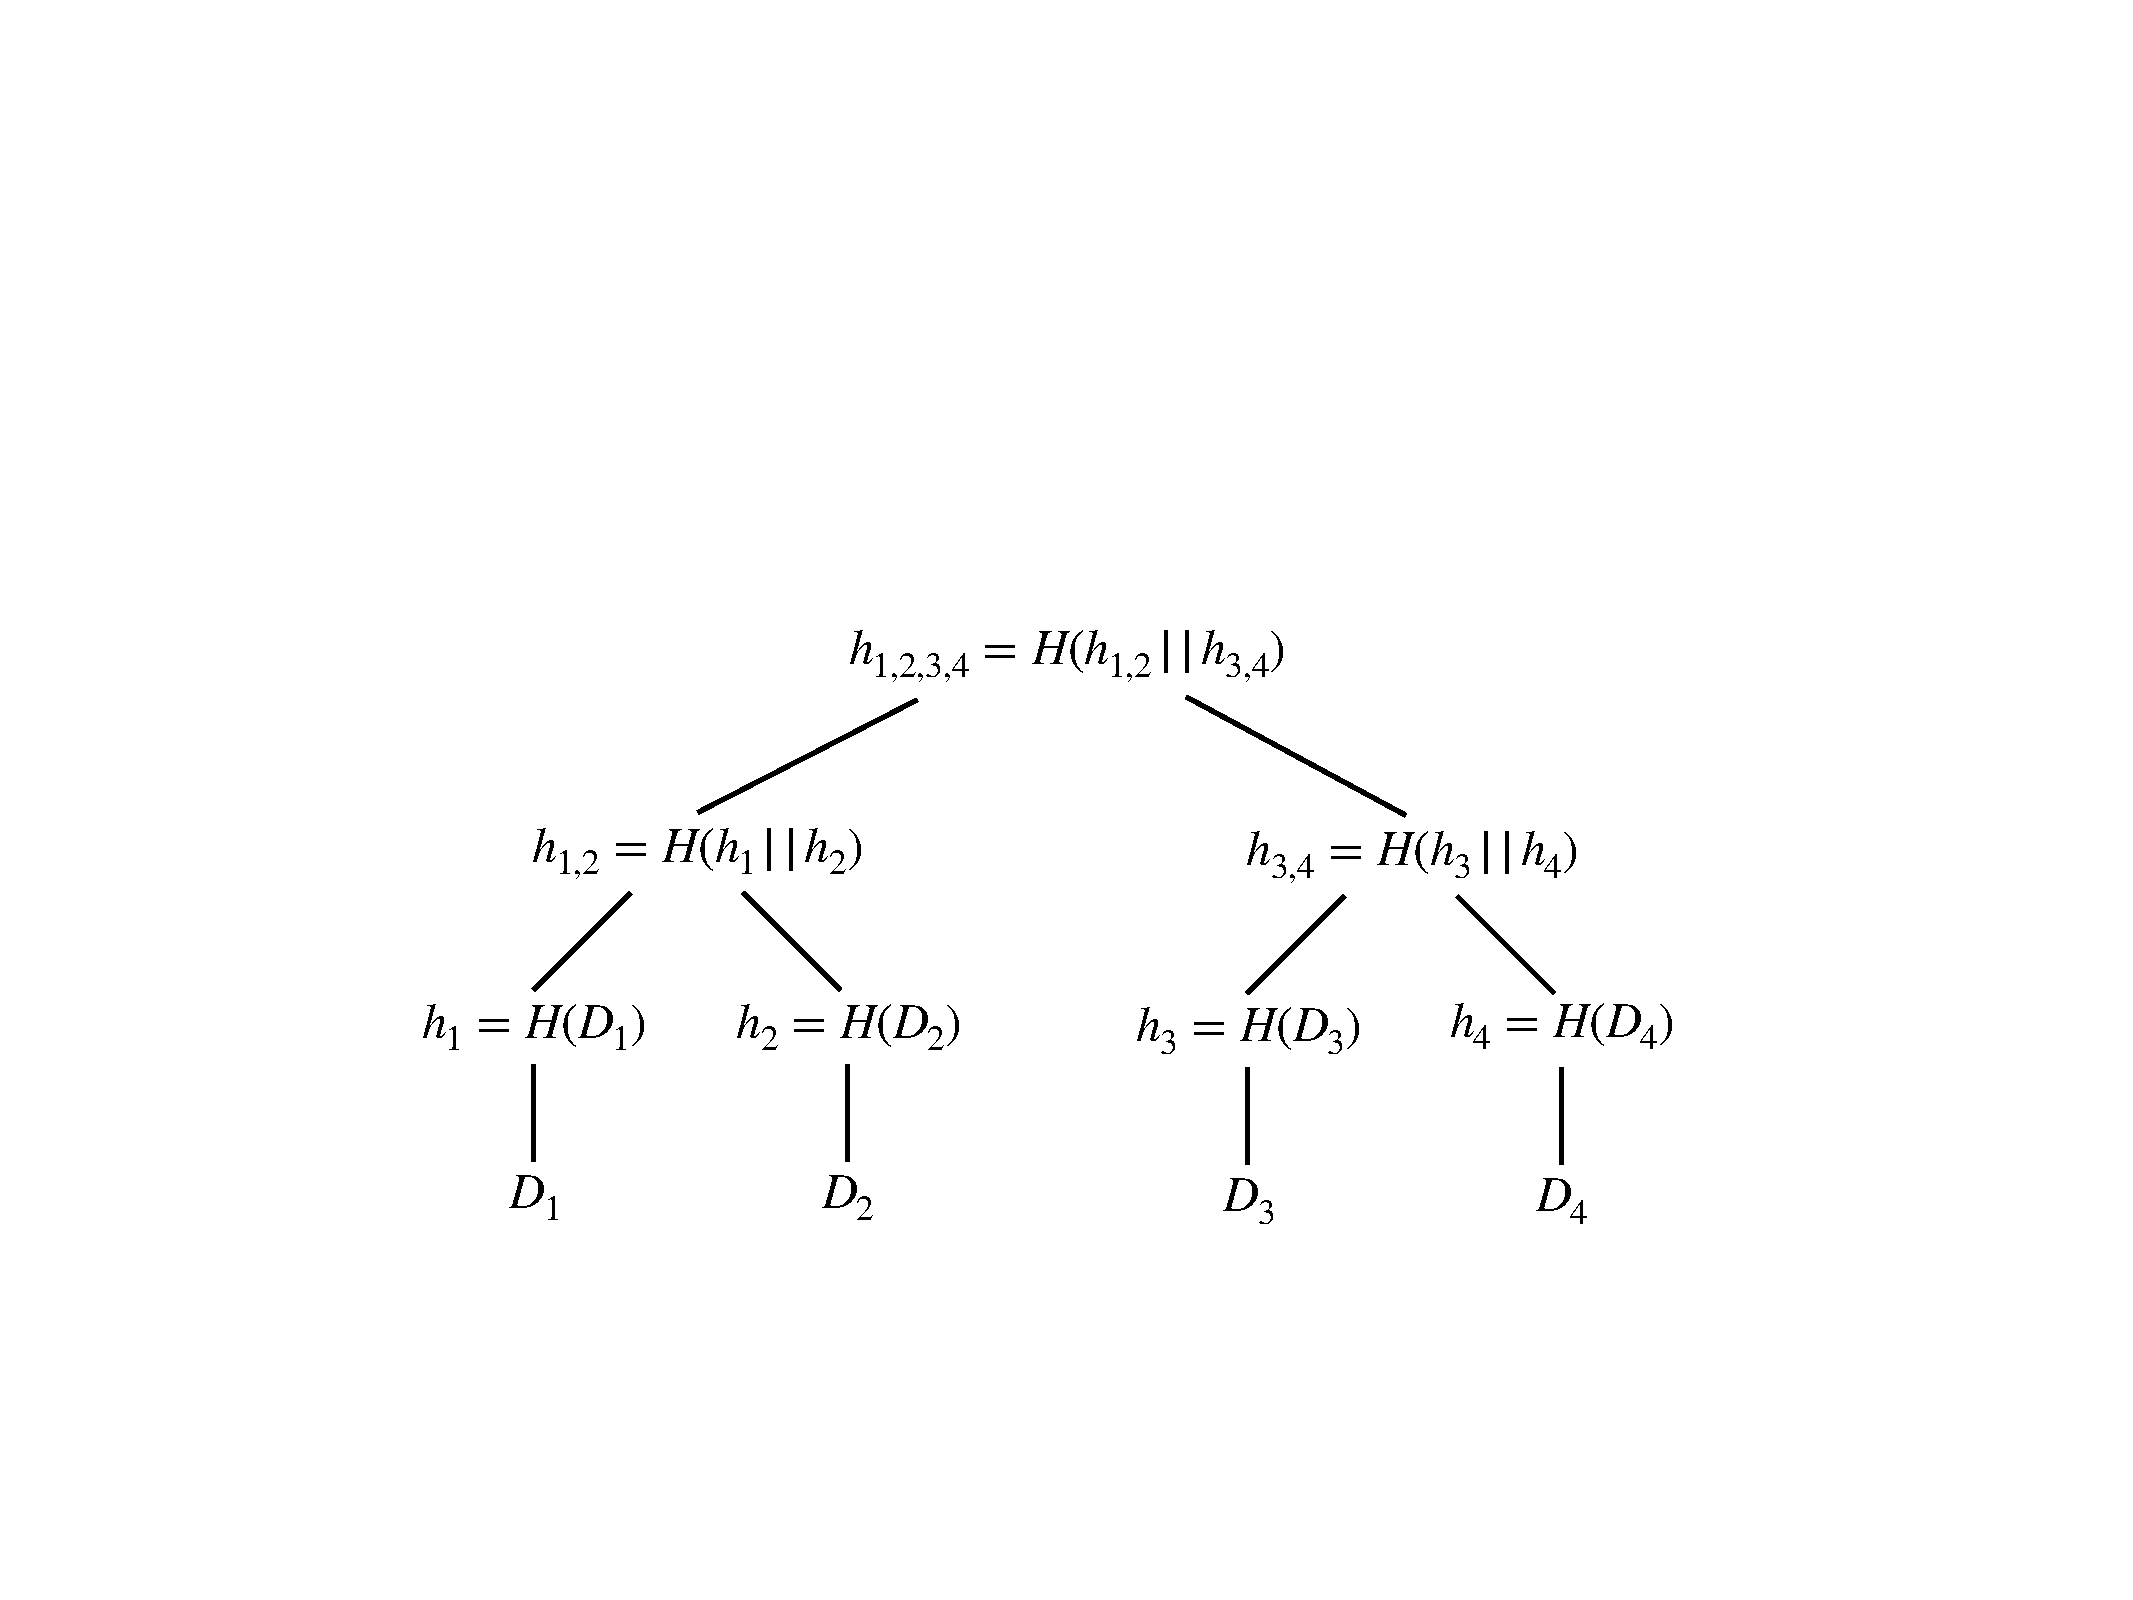
\includegraphics[width=\linewidth]{fig/merkletree}
	\caption{Merkle tree with root $h_{1,2,3,4}$}
\end{figure}

\begin{lem}
If $h_r$ is the root of a Merkle Tree with $n$ data elements, it is possible to proof that $D_i$ is one of the data elements by revealing $D_i$ and $log(n)$ node labels, i.e., hashes.
\end{lem}

\question{What is needed to recompute hashes on a path in the Merkle Tree?
\begin{itemize}
	\item Data position or
	\item Left/right information
\end{itemize}}

\begin{figure}[ht]
	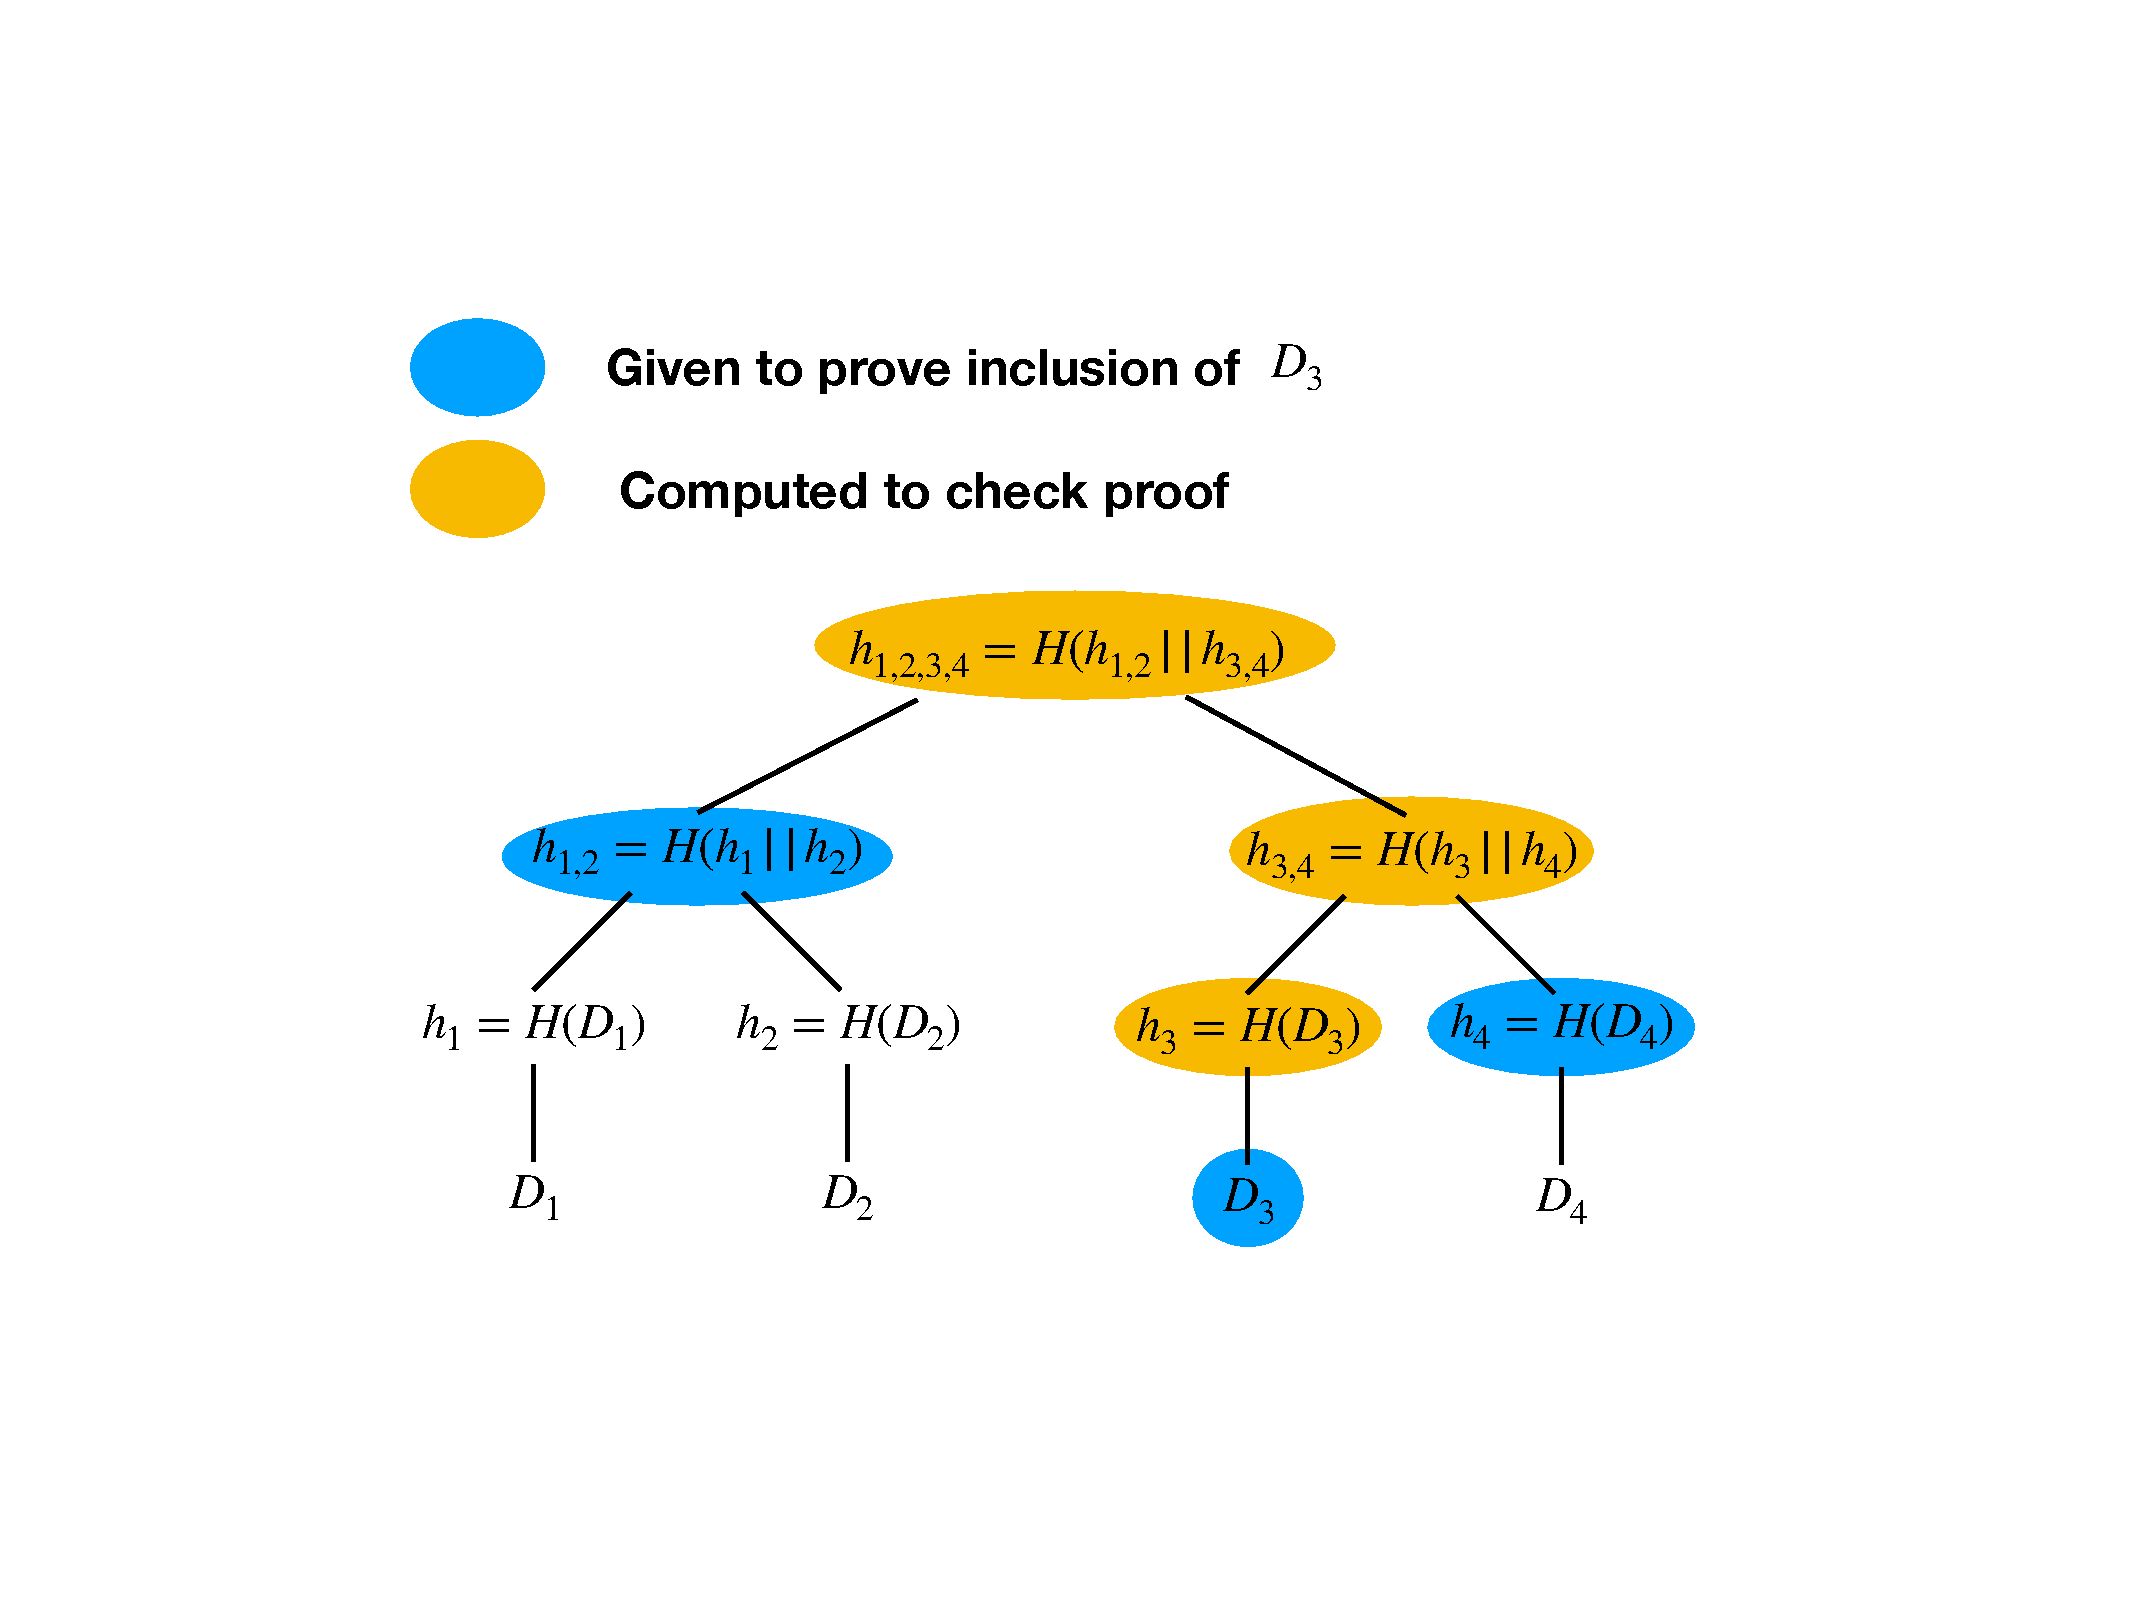
\includegraphics[width=\linewidth]{fig/merkleproof}
	\caption{Hashes necessary and computed to proof inclusion for $D_3$.}
\end{figure}

\question{How many hashes does an inclusion proof contain for a Tree with 3,8,12 or 24 data items?}

\begin{example}
	In a Merkle Tree with 16 data elements, an inclusion proof contains 4 hashes.
	
	In a Merkle Tree with 1000 data elements, an inclusion proof contains 10 hashes.
	
	In a Merkle Tree with 1 million data elements, an inclusion proof contains 20 hashes.
\end{example}

\question{Is it possible to proof that a certain document or peace of data is not included in the Merkle Tree?}

\begin{note}
It is possible to enhance other tree data-structures, e.g. binary search tree or radix tree with hashes from a Merkle tree.
\end{note}

\begin{figure}[ht]
	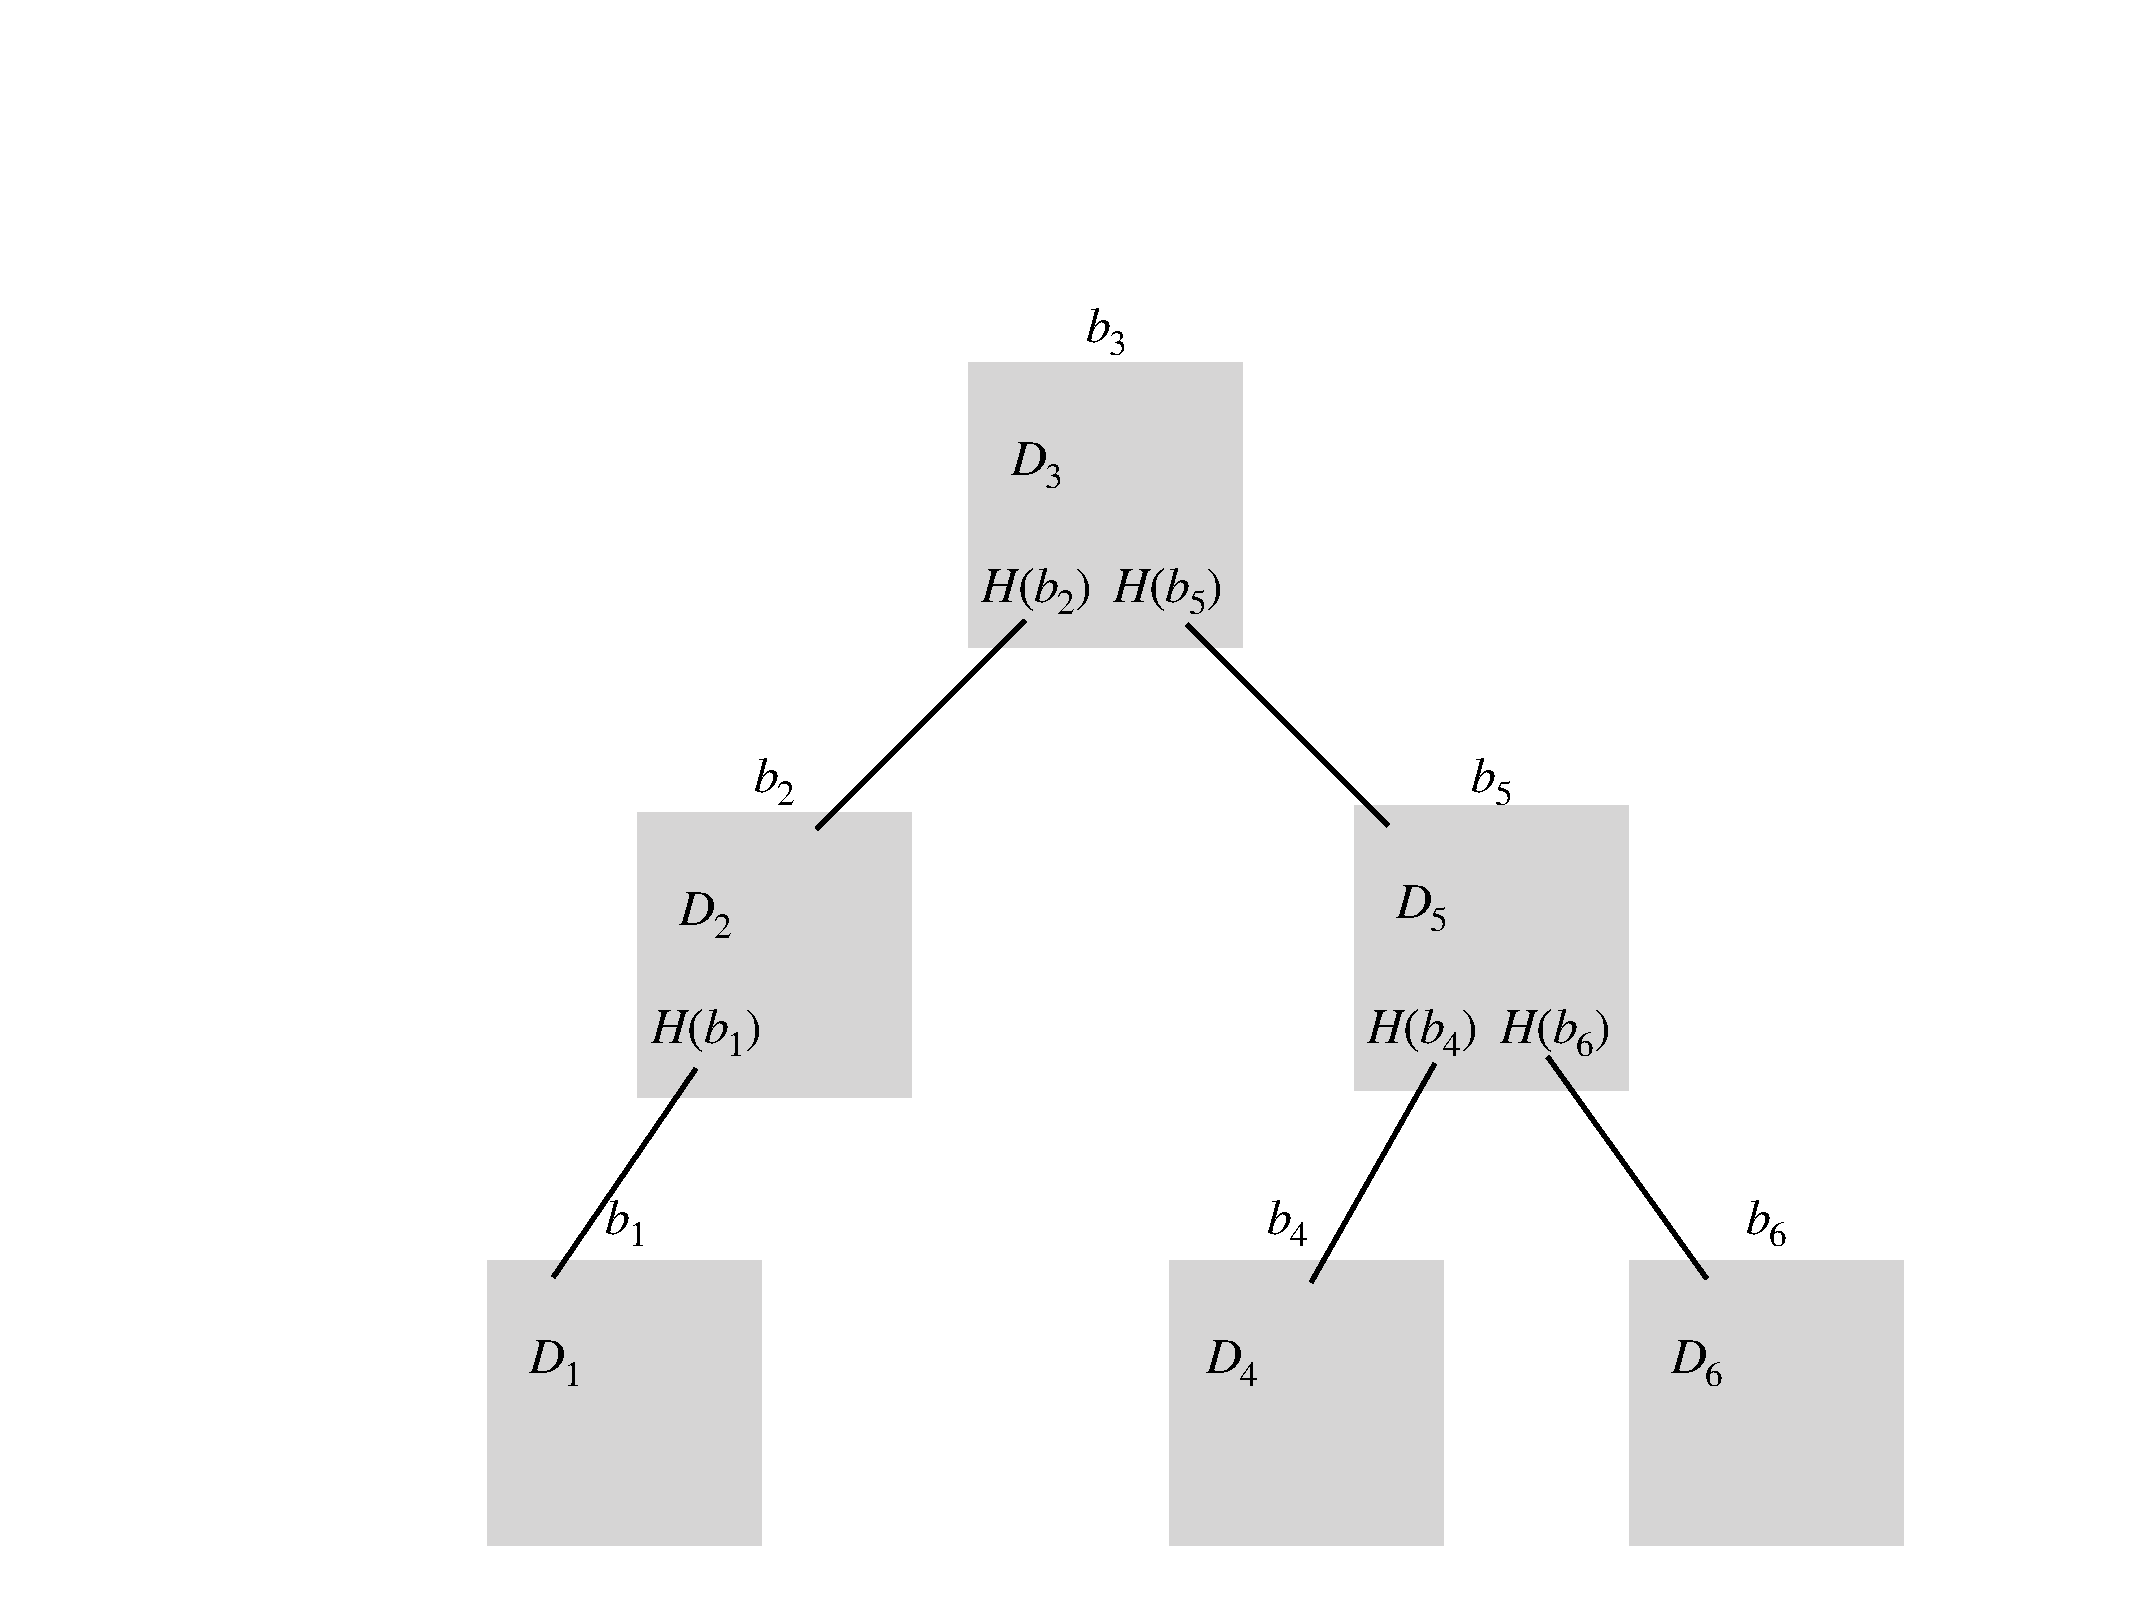
\includegraphics[width=\textwidth]{fig/binarySearchTree}
	\caption{A binary search tree enhanced with hash references.}
\end{figure}

%!TEX root = ../main.tex

\section{Blockchain}
The following blockchain definition combines hash-chain with Merkle trees. 


\begin{definition}\label{def:bc}
A \textbf{Blockchain} is a hash-chain where the data entry in every node is the root of a Merkle tree.
\end{definition}

\begin{note}
	The blockchain construction was not invented for bitcoin. It is used previously in \emph{linked timestamping}, where block headers are published in newspapers.
\end{note}

\question{If the last block header of a blockchain is published, what is necessary to prove that a $D_i$ was data, included in the Merkle tree of the previous block?}

\chapter{Transactions}

%!TEX root = ../main.tex

\section{Digital Signatures}
A short recap of digital signatures.

A signature scheme comprises key generation, signing and verification functions.
Key generation creates a public and secret (private) key pair ($pk, sk$).

Signing function takes an arbitrary message $m$ and the secret key $sk$ and outputs a signature $\sigma$.
\[
\sigma\leftarrow Sign(m,sk)
\]

A verify function takes a message $m$, signature $\sigma$ and the public key $pk$. The verification function returns $\true$, if $\sigma$ was produced for $m$ with the secret key $sk$ matching $pk$. Otherwise verification returns \false.
\[
\{ \true, \false \} \leftarrow Verify(m,\sigma,pk)
\]

Bitcoin currently uses ECDSA signatures, i.e. signatures where the public key is a point on an elliptic curve.

\begin{example}
One example for digital signatures is https certificates and the establishment of a TLS session.
These certify that a given public key belongs to a certain domain.
They are signed by a Certificate authority. 
The public key of the certificate authority is typically already included in your browser installation.

The binding of a public key to a specific entity (e.g. web-domain) is called 
\emph{public key infrastructure} (PKI).
\end{example}

\section{Account balances and UTXO}
The most prominent use case for blockchains is currently digital currency. 
We now spend some time to look at how to implement money transfer. 

\question{How would you implement a digital bank?}

\begin{idea}
	\label{idea-pk}
	We can use public keys as identity for users or owners of money. 
\end{idea}
\begin{note}
Idea~\ref{idea-pk} allows to avoid the use of \emph{public key infrastructure} (PKI), that is otherwise used to bind public keys to identities.
\end{note}

\textbf{Algorithm~\ref{alg:bank}} shows a simple bank that maintains balances.
For every public-key, the bank stores one balance.
The algorithm has two transactions, \textsc{Create} creates new balances.
\textsc{Transfer} allows to transfer money from one account (\textit{pk-from}) to another (\textit{pk-to}.
The algorithm assumes that balances that have not been initialized have the value 0.


\paragraph{Authentication} of transactions poses a problem:
\begin{itemize}
	\item For \textsc{Create} transactions we assume that they are are only valid during setup of the system.
	\item For \textsc{Transfer} transactions it is desired that all transactions can be submitted by users. To authenticate the sender, the transaction includes a signature $\sigma$.
	In Line~\ref{line:if} we therefore check that the sender \textit{pk-from} signed the transaction.
\end{itemize}

\noindent
A bank based on Algorithm~\ref{alg:bank} may be susceptible to \textbf{replay attacks}. A \textsc{Transfer} transaction signed by \textit{pk-from} may be submitted multiple times, given that the account of \textit{pk-from} has sufficient fonds. This will result in additional fonds transferred to \textit{pk-to}.

Later, we will see, how replay attacks in this account based model can be avoided using a counter/sequence number for each account.


\begin{algorithm}[ht!]
	\caption{Simple Bank using account balances}
	\label{alg:bank}
	\begin{algorithmic}[1]
		\State{$balances :=[pk]\textnormal{uint}$}
		\Procedure{Create}{$value, pk$}
			
				\State{$balances[pk] += value$}
			
		\EndProcedure
		\Procedure{Transfer}{$value, \textit{pk-from}, \textit{pk-to}, \sigma$}
			\If{\label{line:if} $\text{verify}(m, \mathit{pk-from}, \sigma)$} 
			\Comment{$m=value||\textit{pk-from}||\textit{pk-to}$}
 				\If{$balances[\textit{pk-from}] > value$ }
					\State{$balances[\textit{pk-from}] -= value$}
					\State{$balances[\textit{pk-to}] += value$}
				\EndIf
			\EndIf
		\EndProcedure
	\end{algorithmic}
\end{algorithm}

\question{How could you implement this bank using a blockchain?}

\begin{note}
\begin{itemize}
	\item[+] Transfer transaction can be submitted by a sender without the receiver being online.
	\item[-] It is possible to (accidentally) send money to a public key that does not exist, i.e. that nobody knows the private key for. 
\end{itemize}
\end{note}

\paragraph{Who runs the bank?}
In a centralized system, a trusted party could process transactions, compute balances and distribute balances to all parties. 

Without a trusted party, it is necessary that transactions are distributed to everybody. Every party can then deterministically compute the balances.

\emph{If all participants get all transactions, they can each process them individually and arrive at the same balances.}


\subsection{UTXO}
Bitcoin does not use balances. Instead it uses the 
\emph{unspent transaction output} (UTXO) model. We now explain this model:

\begin{idea}[UTXO]
In the UTXO model, instead of storing a balance for each private key, we store for every coin, which private key it belongs to. 
This is complicated a bit, since we want to be able to split and merge coins.

Therefore, instead of individual coins, we store unspent transaction outputs, i.e. money received and not yet spend.
\end{idea}

\begin{definition}
	A \textbf{transaction output} is a tuple $(v, pk)$ that shows, that $v$ funds have been transferred. $pk$ is a \emph{spending condition} that must be met to spend claim $v$. Typically $pk$ requires a signature with a given public key.
	
	A \textbf{transaction input} is a tuple consisting of a reference to a transaction output and an argument that meets the outputs condition.
	I.e. $(outp_i,\sigma)$ where $\sigma$ is \emph{redeeming argument} a matching $pk$, e.g. a signature.
	
	A \textbf{transaction} is a tuple containing a list of transaction inputs and a list of new outputs.
\end{definition}


\begin{note}
	\label{bitcoin:transactions}
	In bitcoin transactions are implemented in the following way:
	\begin{itemize}
		\item An output from transaction $t$ is identified by a tuple $(h_t,i)$,
		where $h_t$ is the hash of $t$ and $i$ is the index in the list of outputs in $t$.
		\item Algorithm~\ref{alg:transact} shows how a transaction is validated.
		For a transaction to be valid, \emph{all inputs must be unspent}, input \emph{signatures must validate} and the \emph{sum of input values must be larger than the  output values}.
		\item Algorithm~\ref{alg:transact} ensures that a transaction can only be validated once and no two valid transactions can spend the same output.
		\item The different between transaction inputs and outputs is called transaction \emph{fee}.
		\item Example~\ref{ex:P2PKH} gives an example for more complex conditions that may be required to spend an output.
		\item When the value of inputs is larger than the desired value to be spend, it is common to create an additional output that contains change.
	\end{itemize}
	
\end{note}

\begin{algorithm}[h!]
	\caption{Transaction validation and maintenance of UTXO}
	\label{alg:transact}
	\begin{algorithmic}
		\State{$UTXO := map[(h,i)]\rightarrow(value, pk)$}
		\Procedure{transfer}{$inputs, outputs$}\Comment{Transaction $t$ with hash $h_t$}
			\For{$((h,i),\sigma)\in inputs$}
				\If{$UTXO[(h,i)]$ does not exist}
					\State{\textbf{abort}}
					\Comment{invalid transaction}
				\EndIf
				\If{$\text{verify}(h_t,\sigma, UTXO[(h,i)].pk) == \false$}
					\State{\textbf{abort}}
					\Comment{invalid transaction}
				\EndIf
			\EndFor
			\If{ sum of values of inputs $<$ sum of values of new outputs}
				\State{\textbf{abort}}
				\Comment{invalid transaction}
			\EndIf
			
			\For{$((h,i),\sigma)\in inputs$}
				\State{$UTXO[(h,i)]=nil$} \Comment{output spent}
			\EndFor
			\State{$h_t:= hash(transaction)$}
			\State{$UTXO[h_t]=outputs$}
			\Comment{add new output}
			
			
		\EndProcedure
	\end{algorithmic}
\end{algorithm}

\begin{example}
Alice's public key has two unspent outputs with value 1\$ and 1.5\$. Alice wants to send 2\$ to Bob.
To do that, Alice can create a transaction that has her two outputs as input 
and creates two outputs, one with value 2\$ and Bobs public key. One with value 0.5\$ and Alices public key.
\end{example}


\begin{definition}
A \emph{double-spend} is a situation where multiple transactions attempt to spend the same output. 	
\end{definition}
\begin{note}
Note that according to Algorithm~\ref{alg:transact} only one of double-spend transactions can be validated. 
\end{note}

% \pagebreak


\begin{example}
	\label{ex:P2PKH}
	The following are the most common examples for arguments necessary to claim a transaction output. In Bitcoin they are expressed in a stack based scripting language.
	\begin{enumerate}[label=\alph*)]
		\item A signature that matches a certain public key.
		\item A public key that hashes to a certain value and a signature that matches this key. (Pay to public key hash or P2PKH).
		\item Multiple signatures that match a sequence of public keys. (Multisig)
		\item $m$ signatures that match $m$ out of $n$ provided public keys. 
		E.g. 2 signatures from 2 out of 3 specified public keys.
		\item A script that hashes to a certain value and an argument that causes this script to evaluate to true. (pay to script hash)
	\end{enumerate}
	See \href{https://github.com/bitcoinbook/bitcoinbook/blob/develop/ch06.asciidoc#script-construction-lock--unlock}{Mastering Bitcoin book, Chapter 6, Script Contruction}  and \href{https://d28rh4a8wq0iu5.cloudfront.net/bitcointech/readings/princeton_bitcoin_book.pdf}{Book: Bitcoin and Cryptocurrency Technologies, Chapter~3.2} for explanation of P2PKH script.
\end{example}

\begin{note}
To maintain a copy of our transaction based bank, a node has to maintain the set of all unspent transaction outputs $UTXO$. 

If variant b) is used instead of variant a) from Example~\ref{ex:P2PKH} this may significantly reduce the size of the $UTXO$ data structure. The same holds, if d) is used instead of c).
\end{note}	

\comment{On blackboard, give example of P2PKH script.}

P2PKH makes it possible to pay to the hash of a public key.
This gives rise to the concept of an address.

\begin{definition} An \textbf{address} is either a public key or the hash of a public key. Given the address of a user, it is possible to transfer funds to this user, i.e. create an output that this user can claim by providing a correct signature.
\end{definition}

\begin{note}
Bitcoin and many other cryptocurrencies use Base-58 encoding. This encoding uses small and large letters (a to z) and numbers, omitting 0 (number zero), O (capital o), l (lower L) and I (capital i) because of their ambiguity.

Bitcoin addresses use Base58Check encoding which adds a 4 byte checksum before Base-58 encoding, to protect against typos, ...
\end{note}


\subsection{Privacy in the UTXO model}
\comment{Not covered in lecture}
Different from the account and balance system, the $UTXO$ model encourages the use of different addresses. This makes it harder to identify all transactions done by a single user.

However research has shown, that based on transactions, it is easy to identify different addresses belonging to the same user.

On the other hand, $UTXO$ allows to trace in which transactions a particular value or coin was involved.

\begin{definition}
A \textbf{tainted coin} is a transaction output that is either the result of a transaction considered unethical or illegal or derived from the output of such a transaction by multiple other transactions.
\end{definition}

\begin{note}
Based on the concept of tainted coins it is debatable whether digital cash based on the UTXO model is \emph{fungible}. In economics fungibility is defined as the property that any two units of a good are interchangeable.
\end{note}

\question{What about paper money? Is it fungible?}

The UTXO model allows to create a mixing service:
\begin{definition}
	A \emph{mixing service} can be used to prevent a third party from tracking a specific users transactions. A mixing service would receive payments from many users, and pay them back using new addresses. 
\end{definition}

\begin{note}
	\begin{itemize}
		\item A mixing service makes it hard to see which of the new addresses belongs to which of the users that sent money to the mixing service.
		\item A mixing service usually requires a high fee.
		\item A mixing service is usually implemented as a centralized entity.
	\end{itemize}
\end{note}

\chapter{Proof of work}
%!TEX root = ../main.tex

In this chapter we discuss how the Transactions, introduced in 
Chapter~\ref{ch:transaction} are included in a block in the hash-chain,
introduced in Chapter~\ref{ch:hashchain}.

\section{Centralized straw-man system}
We present a straw man solution that relies on a centralized leader to include transactions into a block and issue those blocks. 
After discussing difficulties with this approach, we present the proof of work based scheme used in bitcoin.

As shown in Figure~\ref{fig:leader}, we assume a single leader. Transactions are submitted to the leader and included in a block.
The block is then broadcast to all participating nodes, who validate it.
\emph{The validation of blocks prevents the leader from including malformed transactions}, however this system still opens several ways for the leader to misbehave:
\begin{enumerate}[label=\Alph*)]
	\item The leader can omit certain transactions on purpose. (Censorship)
	\item The leader is a single point of failure.
	\item The leader could send different blocks to different processes.
\end{enumerate}
\comment{If bitcoin would have a leader, some agency would have shut it down long ago.}

\begin{figure}
	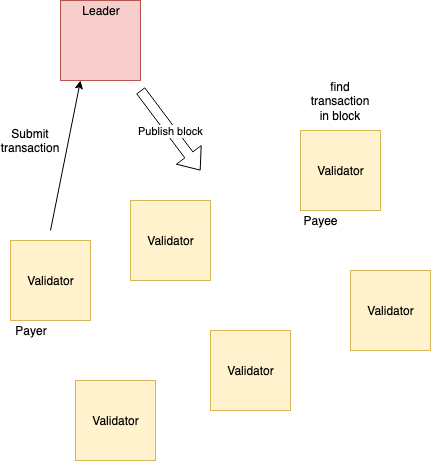
\includegraphics{fig/Leader}
	\caption{Straw-man system with leader}
	\label{fig:leader}
\end{figure}

\pagebreak
\section{PoW function}

\begin{definition}\label{def:pow1}
	(PoW function version 1)
	For an integer $d$,
	the proof-of-work (PoW) function with difficulty $d$ takes a data item and returns a nonce (random bits) and a hash value:
	\[
		(h_{PoW}, nonce)=f_{PoW}(Data)
	\]
	The proof of work is \emph{valid}, if a) $h_{PoW}$ is the hash of the data, concatenated with the nonce
	\[
		h_{PoW} \overset{?}{=}H(Data || nonce))
	\]
	and b) the first $d$ bits of $h_{PoW}$ are 0.
\end{definition}

\begin{note}
	The function $f_{PoW}$ is computed by choosing a random $nonce$ and checking if the condition b) holds. If it does, we also say that the $nonce$ 
	\emph{solves} the proof of work.
\end{note}

The following is an important conclusion. It follows since the result of hashing one data item is independent from hashing another data item.

\begin{lem}\label{lem:independent}
	Given two $nonces$, chosen at random. 
	The probability that any of them solves the proof of work is independent.
\end{lem}


\question{If we require $d$ initial 0, what is the probability $p$? What is the expected number of trials?}

\begin{theorem}
	\label{thm:bernoullitrials}
	If we conduct multiple, independent Bernoulli trials with success probabilty $p$, the expected number of trials necessary until success is $\frac{1}{p}$. 
\end{theorem}

For proof see \href{https://cut-the-knot.org/Probability/LengthToFirstSuccess.shtml}{here}.

\question{If we require $d$ initial 0, what is the expected number of trials until success?}

\question{Assume for $d=11$ the expected time until success is 7 minutes. What is the expected time until success for $d=10$ and $d=12$?}

\begin{note}
Using version 1 of the proof of work function, adjusting $d$ the difficulty of the proof of work can only be doubled or halved.
\end{note}

\begin{definition}\label{def:pow}
	(PoW function version 2)
	For an hexadecimal number $d$,
	the proof-of-work function with difficulty $d$ takes a data item and returns a nonce (random bits) and a hash value:
	\[
		(h_{PoW}, nonce)=f_{PoW}(Data)
	\]
	The proof of work is \emph{valid}, if a) $h_{PoW}$ is the hash of the data, concatenated with the nonce
	\[
		h_{PoW} \overset{?}{=}H(Data || nonce))
	\]
	and b)  $h_{PoW}$ written as hexadecimal number is smaller than $d$.
	\[
		h_{PoW} < d
	\]
\end{definition}

\question{Which $d$ in definition \ref{def:pow} gives that valid solutions all have $16$ initial 0 in bit representation?}

\begin{note}
	The proof of work function from Definition~\ref{def:pow} allows to carefully adjust the difficulty $d$ to achieve a certain expected time.
\end{note}

\section{Block creation with PoW}

\begin{idea}
	The idea behind block creation using PoW is to require that any block published includes a nonce, s.t. the block hash and nonce are results of a PoW function.
	
	We then allow every node to publish a block, if it can find a valid proof of work.
\end{idea}

\begin{definition}
A \emph{proof of work blockchain} is a blockchain as in Definition~\ref{def:bc} where additionally, every block contains a $nonce$ and the hash of the previous block hash $h_{-1}$, the root of the merkle tree and the $nonce$ solves the difficulty.	
\end{definition}

\begin{figure}
	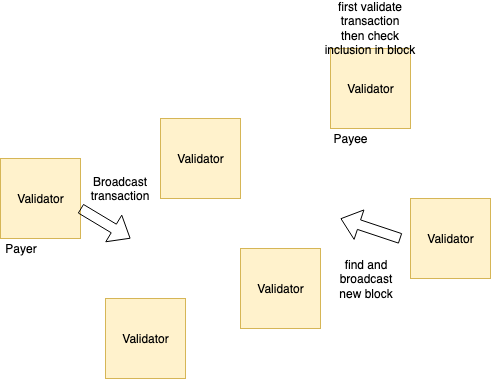
\includegraphics[width=\linewidth]{fig/NoLeader}
	\caption{Block creation with PoW}
	\label{fig:leader}
\end{figure}

\begin{description}
	\item[Censorship] An adversary cannot prevent a node, it does not control from including a certain transaction.
	\item[Failures] Failure of individual nodes will not prevent the system from running.
	\item[Frequency] PoW difficulty can be adjusted, to ensure that a block is broadcast to everybody, before the next block arrives.
	\item[Conflicting blocks] For a single entity to create two different blocks at requires to solve PoW twice. This makes it difficult to publish two conflicting blocks.
	A high difficulty decreases the probability that two blocks are found concurrently.
\end{description}

\subsection{Adjustable difficulty}
Back in 2010 it was possible to join Bitcoin and create a new block using a simple desktop computer. Today specialized hardware (ASICs) is used to solve the PoW.
\begin{idea} To adjust to nodes joining and leaving the system, and nodes using different infrastructure (i.e. hardware) it is possible to adjust the hardness of the blockchain.
\end{idea}

\begin{definition}
Additional to the merkle root and nonce Bitcoin includes a timestamp in the	block (and in the PoW). This allows to compute the average time between two blocks every 2016 blocks and adjust the difficulty.
\end{definition}

\begin{note} on timestamps in a PoW blockchain
	
\begin{itemize}
	\item The time between blocks can vary significantly but this variance has little effect on the average time, taken over 2016 blocks.
	\item The timestamp can be set by the nodes when creating the block. When validating the block nodes check that the new block has a timestamp within 2 hours of their local clock.
\end{itemize}
\end{note}

\begin{lem}
	If we assume that the probability that the nodes find a new block within time $\Delta$ is constant and independent, and assume that the mean time to block creation is 10 minutes, we can compute the probability, that a block is created within $t$ seconds as
	\[
		P[\text{block created within } t \text{ seconds}] = 1- \left(\frac{599}{600} \right)^t
	\]
	\[
		P[\text{no block created within } t \text{ seconds}] = \left(\frac{599}{600} \right)^t
	\]
\end{lem}
\begin{proof}
Let $p$ be the probability that a block is found within 1 second.
Let $T$ be the random variable describing after how many seconds a new block is found. Since finding a block in a specific second is independent we get:
\[
P[T=t] = (1-p)^{t-1}p
\]
From Theorem~\ref{thm:bernoullitrials} it follows that $E[T] = \frac{1}{p}$.
If we assume $E[T]= 10 \text{min} = 600$ we get $p=\frac{1}{600}$.
\end{proof}

\question{What is the probability that a block is found in:
\begin{itemize}
	\item Less than 3 minutes?
	\item Less than 1 minute?
	\item Less than 10 minutes?
	\item More than 15 minutes?
	\item More than 30 minutes?
\end{itemize}
Why is the probability for less than 10 minutes not 0.5?
}

\subsection{Fees and mining rewards}
Fees and mining rewards give an incentive to solve the PoW function.

\begin{definition}
When the sum of outputs of a transaction is larger than the sum of inputs, the difference is called \emph{fee}.	
\end{definition}

\begin{definition}
 Every block in bitcoin contains a \emph{coinbase transaction}. This transaction has no input and a single output. The output value is the sum of a fixed reward (\emph{mining reward}) and the sum of all fees of transactions included in the block.
\end{definition}

\begin{note} There are different \textbf{pro's and con's for fixed rewards and fees:}
	\begin{itemize}
		\item In bitcoin the mining reward is halved every 4 years. Thus, only a finite amount of bitcoin will ever be created.
		\item The mining reward allows cheap transactions, since fees do not need to cover full mining expenses.
		\item Some research suggests, that if mining rewards are small compared to fees, mining becomes unstable.\footnote{\url{https://freedom-to-tinker.com/2016/10/21/bitcoin-is-unstable-without-the-block-reward/}}
		\item Mining awards are necessary to get money into circulation.
	\end{itemize}
\end{note}

\question{How to determine fees? Banks/credit cards often take percentages.}

\begin{note} \textbf{How big should the fee be?}
Fees are determined by market economics, i.e. nodes choose which transactions to include. Usually those with highest fee.
	
Processing of transactions requires nodes to use network and processing capacities (for relaying and validating transactions). These expenses depend on the size of a transaction, but not on the value transferred. Therefore:
\begin{itemize}
	\item Fees in bitcoin are usually independent of the value of a transaction. Instead they depend on the size (in bytes) of the transaction.
\end{itemize}
\end{note}

\subsection{Forks and longest chain rule}
As mentioned above, PoW can reduce the probability for conflicting blocks to be proposed, but cannot prevent this from happening.

\begin{definition} A \emph{fork} in a blockchain is when multiple blocks are proposed with the same predecessor. Note that every block in a fork may be extended to a different chain.
\end{definition}

A fork is problematic since the different blocks or chains represent two versions of the world. 
	
\emph{Imagine your bank being undecided, wether you did or did not payed your rent.}

\begin{definition} (Longest chain rule) If a fork exist should adopt the longest chain.
\end{definition}

\begin{note} While the Longest chain rule is implemented in the standard bitcoin release, it is not enforced. It is possible to extend a different chain than the given by the longest chain rule. Doing this may change what is the longest chain. 
\end{note}

\begin{lem}
	Given two chains $c_1$ and $c_2$. To find a new block extending $c_1$ is equally likely as finding a new block extending $c_2$. This even holds, if nodes already spend significant resources to find a block extending $c_1$.
\end{lem}
\begin{proof} This follows from Lemma~\ref{lem:independent}.
\end{proof}

\begin{lem}
Assume two chains $c_1$ and $c_2$ where $c_1$ is longer than $c_2$. Further assume that most nodes follow the longest chain rule, trying to extend the longest chain.
	A new block is more likely to be eventually part of the longest chain, if it is added to $c_1$ rather than $c_2$.
\end{lem}
\begin{proof}
Chain $c_1$ is already longer than $c_2$. A new block would make $c_1$ even longer, while it would make $c_2$ at most equally long to $c_1$.
\end{proof}

\section{PoW and network latency}
We now analyze the probability that a fork occurs based on the network delay, i.e. the time it takes to broadcast a block to the different nodes.

\begin{definition}
	We write $\delta$ for the average time it takes for a block until it is validated by a specific node in the network.
\end{definition}

\begin{note} Based on empirical evaluations, in the current bitcoin network, $\delta=12.6$ seconds. 
\end{note}

In the following theorem we assume that nodes have the same mining power and are following the longest chain rule.
\begin{theorem}
	Let $p$ be the probability that a block is found within one second.
	Then the probability for a fork is
	\[
		1-(1-p)^\delta
	\]
\end{theorem}
\begin{proof}
The probability for a fork is the probability that the while the block is propagated, another block is found.
Thus $$P[\text{fork}] = 1- P[\text{no block found during dissemination}]$$

$$P[\text{no block found during dissemination}] = (1-p)^\delta$$
\end{proof}

\begin{cor}Let $P[\textnormal{fork}^l]$ be the probability that after a fork, both chains are extended by $l$ blocks. It holds
	\[
		P[\textnormal{fork}^l] \leq \left(1-(1-p)^\delta\right)^l
	\]
	
\end{cor}

\question{
\begin{itemize}
	\item What is the probability for a fork in bitcoin?
	\item What is the probability that a fork extends for two blocks?
	\item What is the fork probability if the average network delay $\delta$ is 1 minute?
	\item What is the fork probability if the average block delay is 1 minute or 10 seconds?
\end{itemize}

}
	
%!TEX root = ../main.tex

\section{Attacks on bitcoin mining}
In Section~\ref{sec:fork} we have shown that continued forks are
extremely unlikely, if nodes stick to the longest chain rule and
do not disturb the network latency.

In the following we first look at two ways to deviate from the 
longest chain rule, stubborn mining and selfish (hidden) mining.
And we look at network attacks that might be performed.

We first look at those attacks from the perspective of fair mining.
Then we look at them from the perspective of a double spend.

\begin{definition}
Mining, or block creation is \emph{fair} if a node that possesses $\alpha$ 
percent of the hashing power in the network ends up publishing $\alpha$
blocks in the longest chain.
\end{definition}


\subsection{Stubborn mining}
A node does perform stubborn mining, if it does not abandon the 
current chain for the longest chain. Thus it does not follow the longest chain rule.

More precisely, if there exist two blockchains $c_1$ and $c_2$ 
and $c_2$ contains one more block than $c_1$. Thus the initial state is as shown in Figure~\ref{fig:fork}.
A stubborn node that has published a block in $c_1$ that is not
part of $c_2$ will continue to try and extend $c_1$ until either
$c_1$ becomes the longest. We assume that if the difference between
$c_1$ and $c_2$ increases, the stubborn node will abandon $c_1$.

\begin{theorem}
	
	Stubborn mining does not increases the expected outcome of a node, if
	the node controls less than $\alpha=0.42$ of the hashing power in the network.
	
\end{theorem}
\begin{proof}
	We model this system as a markov chain with 4 states.
	\begin{itemize}
		\item[Loose] where chain $c_1$ was extended faster than $c_2$.
		\item[$-1$] where chain $c_1$ is one block longer than chain $c_2$.
		\item[$0$] where $c_1$ and $c_2$ are equally long.
		\item[Win] where chain $c_2$ became the longest chain.
	\end{itemize}
	
	We ignore the probability that additional forks occur on $c_2$ but 
	note that they would increase the profitability of stubborn mining.
	Assume the probability that the attacker finds a block is $\alpha$,
	while $\beta=1-\alpha$ is the probability that the remaining miners find a block. The states and the transition probabilities are shown in Figure~\ref{fig:stubborn}.
	\begin{figure}
	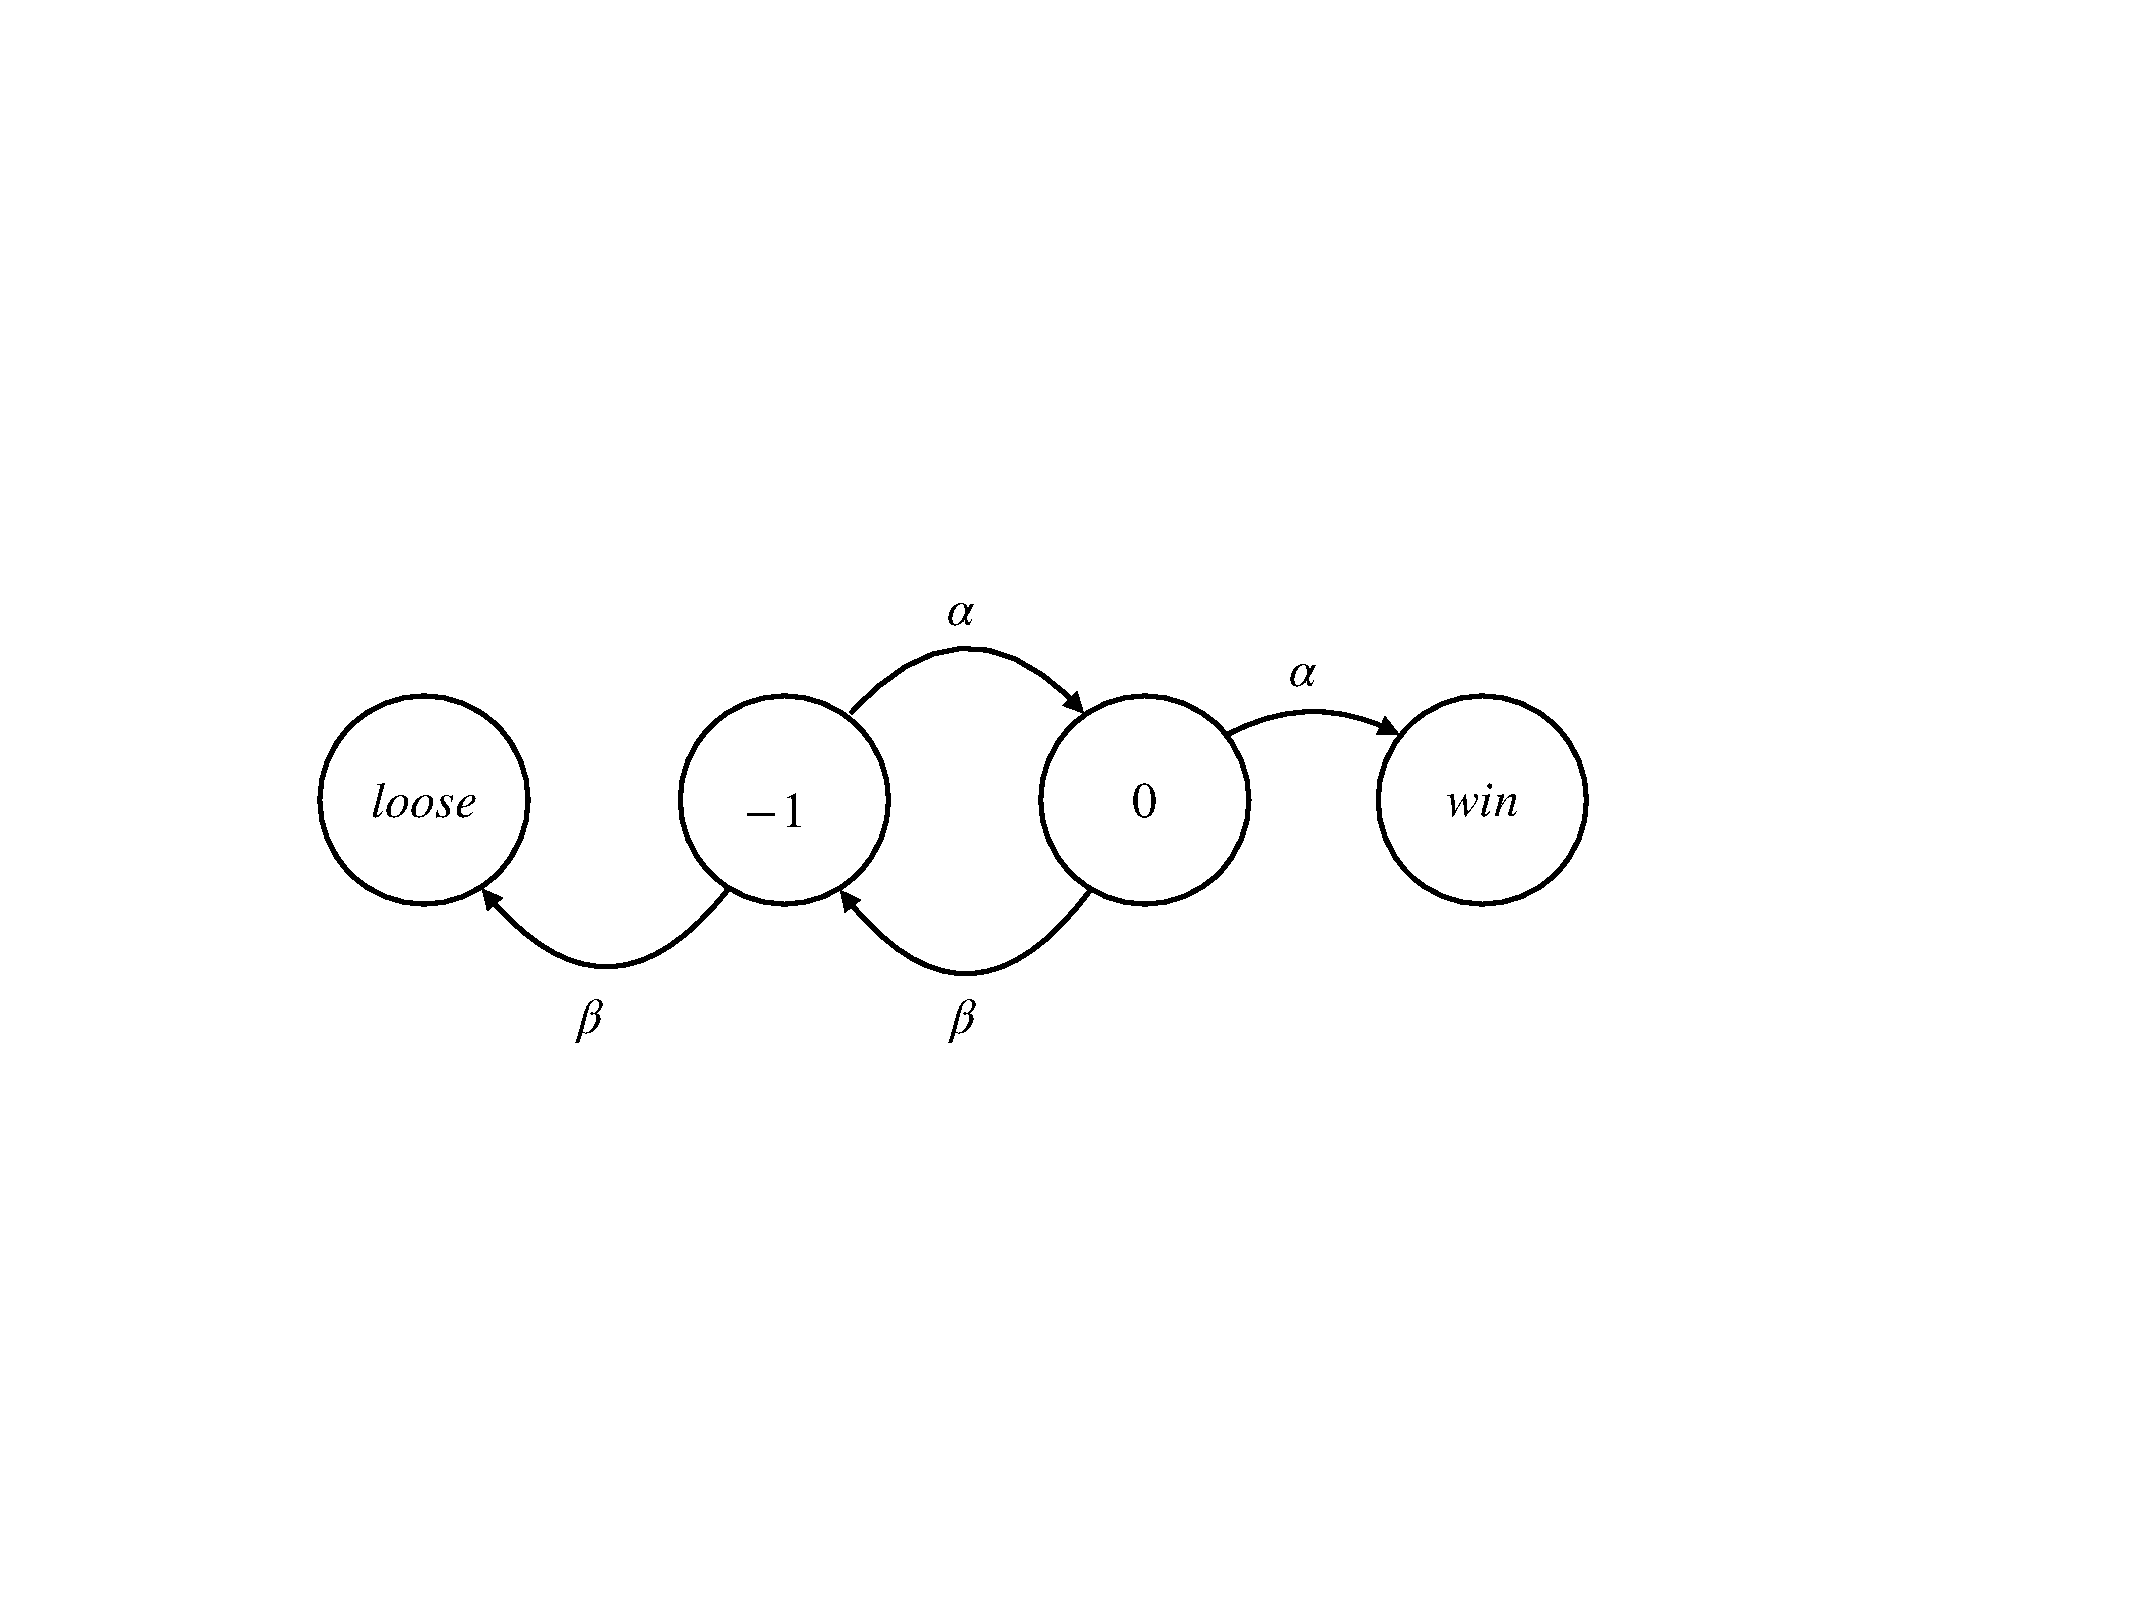
\includegraphics[width=\textwidth]{fig/StubbornMining}
	\caption{Stubborn mining states and transitions.}
	\label{fig:stubborn}
	\end{figure}
	
	We now calculate the expected number of blocks the Attacker receives with and without doing the attack. 
	For the attack we consider the following cases:
	\begin{itemize}
		\item With probability $\beta$ the attacker loses in the first step and receives no blocks.
		\item With probability $\alpha\cdot \alpha$ the attacker mines two blocks. He receive 3 blocks in total.
		\item With probability $\alpha\cdot\beta\cdot \alpha\cdot \alpha$ the process goes through states $-1\mapsto 0 \mapsto -1 \mapsto 0 \mapsto win$.
		In this case the attacker gets 4 blocks.
	\end{itemize}
	Extending the above cases, and omitting those that give 0 blocks,
	$E_{Attack}$ the expected number of blocks is:
	\begin{align}
		E_{Attack}&=\sum_{i=0}(i+3)\alpha^{i+2}\beta^{i}\\
				  &=3\alpha^2+\alpha\beta\left(\sum_i=0(i+3)\alpha^{i+2}\beta^i +\sum_{i=0}\alpha^{i+2}\beta^i\right)\\
				  &=3\alpha^2+\alpha\beta\left(E_{Attack} +\frac{\alpha^2}{1-\alpha\beta}\right)
	\end{align}
	In step (3.2) we used the formula for a geometric sum.
	Solving the above for $E_{Attack}$ gives
	\[
		E_{Attack}=(3+\alpha\beta)\frac{\alpha^2}{1-\alpha\beta}
	\]
	
	To compute the average number of blocks, the attacker would receive if it did not follow the attack, we note that the he gets one block every time an edge with probability $\alpha$ is traversed. We get the following cases.
	\begin{itemize}
		\item With probability $\alpha\cdot \alpha$ the node mines two blocks.
		\item With probability $\alpha\cdot\beta\cdot \beta$ the process goes through states $-1\mapsto 0 \mapsto -1 \mapsto loose$. The node mines 1 block.
		\item With probability $\alpha\cdot\beta\cdot \alpha\cdot \alpha$ the process goes through states $-1\mapsto 0 \mapsto -1 \mapsto 0 \mapsto win$.
		In this case the node gets 3 blocks.
	\end{itemize}
	Continuing the above analysis, we see that the average number of blocks received when not following the above state machine, but not following the attack, is:
	\[
	E_{NoAttack}=\sum_{i=0}(i+2)\alpha^{i+2}\beta^i + \sum_{i+0}i\beta^{i+1}\alpha^i
	\]
	Using the same techniques as for $E_{Attack}$, we get:
	\[
	E_{NoAttack}=(2+\alpha\beta)\frac{\alpha^2}{1-\alpha\beta}+(1+\alpha\beta)
	\]
	
	Plotting both graphs we see that $E_{Attack}<E_{NoAttack}$ holds approximately for $\alpha<0.42$.
\end{proof}

\subsection{51\% attack}
If a miner owns $\alpha=51\%$ of the hashing power in the network, he can attack the network by creating and growing his private chain.
Key to this attack is that the attacker will be able to grow his private chain faster than the remaining network can grow the public chain.

\begin{example}
This example is shown in Figure~\ref{fig:51}. 
Assume at the begin of the attack the longest chain contains blocks $b_1$, $b_2$, and $b_3$. The attacker picks a recent block, e.g. $b_2$ and starts secretly extending $b_2$. Once the attacker has extended his chain longer than the public chain he can publish it and all blocks in the public chain will be discarded.
\end{example}

\begin{figure}
	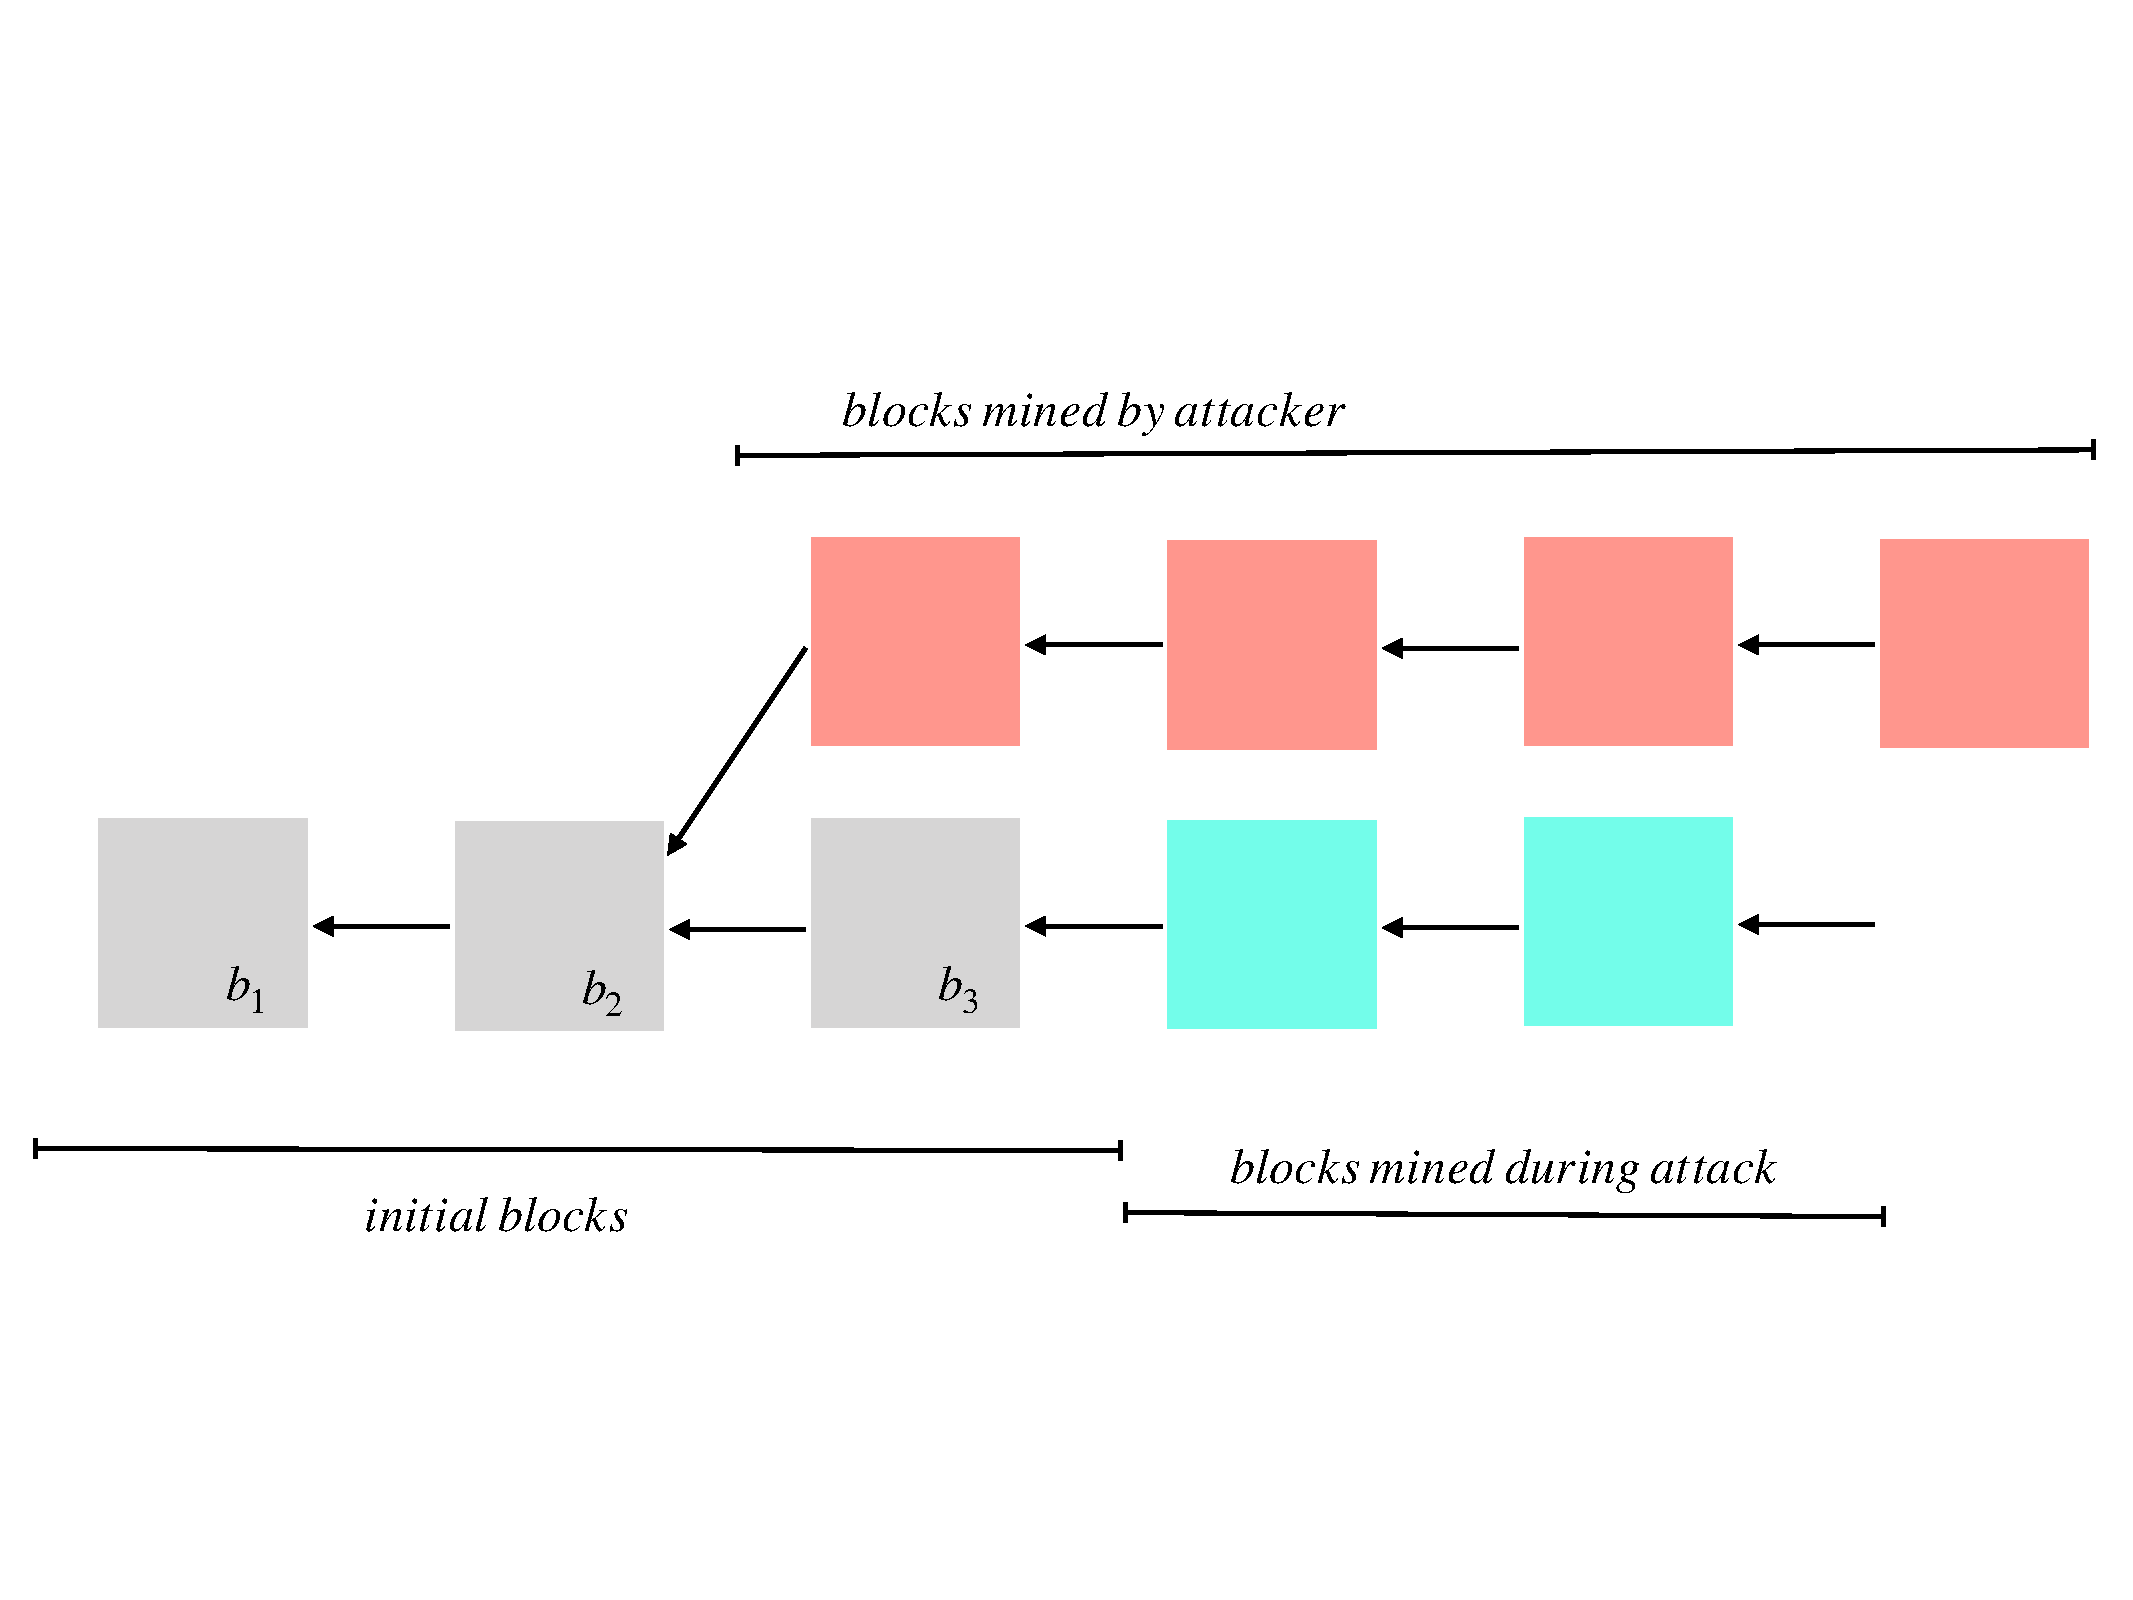
\includegraphics[width=\textwidth]{fig/51attack}
	\caption{A 51\% attack.}
	\label{fig:51}
\end{figure}

\subsection{Selfish mining}
In a selfish mining attack, the attacker does not violate the longest chain rule. Instead he violates the following mandate:
\begin{description}
	\item[Publication mandate] When a node finds a block, it should immediately announce this to the other processes. 
\end{description}
The idea behind not publishing the newest block is that it denies the other nodes to try and extend the longest chain. Thus, other nodes waist resources, trying to extend a chain, that is not the longest chain.

For a detailed description and analysis of selfish mining see 
 \href{https://disco.ethz.ch/courses/distsys/lnotes/chapter26.pdf}{Chapter 26.1} of these Lecture notes form ETH Zurich.
 
\begin{note}
Results above show, that, if the attacker has more than $1/3$ of the hashing power, he can increase the ratio of blocks he creates in the blockchain by selfish mining.

\begin{itemize}
	\item If the attacker has more than $\alpha=1/3$ of the hashing power, he can increase the ratio of blocks he creates in the blockchain by selfish mining.
	\item If the attacker has more than $\alpha=1/4$ of the hashing power, and can reach $\gamma=0.5$ half of the nodes before another miner can reach them, he can benefit from selfish mining.
\end{itemize}
\end{note}

\section{P2P networking and network layer attacks}
A node in bitcoin does not maintain connections to all 10.000 bitcoin nodes.
Instead every node maintains a membership list, with addresses of other nodes. He maintains connections only to a few nodes selected at random from the list. 
We say that these connections form an overlay network.

In Bitcoin, nodes per default start by establishing 8 connections and extend this to up to 125 connections.

When a block is broadcast, every peer receiving the block first validates it and then forwards it to its neighbors. 

\subsection{Inventory messages and delivery denial attack}
The forwarding of a block consumes significant bandwidth. 
Bitcoin therefore uses \textsc{Inventory} messages to announce the a block to neighbors. Receiving an \textsc{Inventory} message a node would request to receive the actual message from only one of its neighbors. 

Nodes set a timeout when requesting a block. If they do not receive the block within the timeout, it is requested from a different source.

\begin{itemize}
	\item In bitcoin version 0.10, the timeout for receiving a block is set to 20 minutes.
\end{itemize}

\begin{definition}
In a \emph{delivery denial attack} a node does send \textsc{Inventory} messages, but when a block is requested, does not forward the block.	
\end{definition}

For extended details on this attack, see \href{https://scalingbitcoin.org/zh_HANS/papers/bitcoin-block-transaction-delivery.pdf}{[Gervais et. al. in CSS'15]}.
\question{What is the effect of this attack?}

\begin{note}
	Due to the static timeout, a delivery denial attack can significantly slow down block propagation.
	
	\begin{itemize}
		\item Slowing delivery of blocks increases the probability of a fork, as can be seen from Theorem~\ref{thm:fork}. This also increases the probability that a fork extends for several blocks.
		\item Slowing delivery of competing blocks may increase parameter $\gamma$ in the selfish mining scheme and thus make selfish mining more appealing and profitable even when $\alpha<1/4$.
	\end{itemize}
	
\end{note}

\subsection{Eclipse attack}




\section{Updating a blockchain}

\section{Pow as voting}

\chapter{Alternative PoW}
%!TEX root = ../main.tex

\section{Improving PoW}



\subsection{Alternative mining puzzles}
See Chapter 8 of \href{https://d28rh4a8wq0iu5.cloudfront.net/bitcointech/readings/princeton_bitcoin_book.pdf}{this book}.

\begin{definition}
A suitable mining function has the following properties:
\begin{description}
	\item[Adjustable difficulty] It must be possible to adjust the difficulty to adapt to a growing network.
	\item[Fast verification] Every node in the network needs to verify a solution. Thus verification should be easy, compared with computation.
	\item[Progress free] The probability to solve the PoW function in the next second, should be independent of how long a process has been trying to solve it.
\end{description}
\end{definition}


\subsection{ASIC resistance}
Asics resistance is motivated by the fact that bitcoin mining is currently done almost exclusively on specialized hardware, i.e. application specific integrated circuits (ASICs). There are currently produced by a single manufacturer, yielding a single point of failure and trust. 

Further, these ASICs are difficult to use for other purposes than mining cryptocurrencies.

\begin{definition}A PoW puzzle is \emph{ASICs resistant}
if specialized hardware can only provide a small benefit in computing this puzzle, compared to a general purpose CPU.
\end{definition}

\begin{note}
	Proposals for ASICs resistant puzzles include
	\begin{description}
		\item[Memory hard functions] The idea for this is to design puzzles that require a lot of memory access. The idea is that memory access is harder to optimize than cpu computation, as done for hashing.
		\item[CPU benchmarks] A recent proposal~\href{https://conferences.computer.org/icdcs/2019/pdfs/ICDCS2019-49XpIlu3rRtYi2T0qVYnNX/7v1qCHBMZ7kt9TX7Q7GlHe/6ND9kaBwjCCoPVJQvvyQ81.pdf}{HashCore ICDCS'19} proposes to use CPU benchmarks, used normally during hardware development, to create PoW puzzles.
	\end{description}
Both proposals result in functions that are harder to verify.
\end{note}

\subsection{Proof of useful work}
The idea behind proof of useful work, is that energy and hardware used to compute PoW solutions seems "wasted".

\begin{definition} A PoW puzzle is \emph{useful}, if its solution or computation has an application or utility outside of blockchain domain.
\end{definition}

\begin{note} Proposals for useful PoW are still subject to research. Proposals include:
	\begin{description}
		\item[Finding prime numbers]
		\item[Evaluate small degree polynomials] This can help to determine mathematical problems like vector orthogonality, shortest path problems, ...
	\end{description}

Note that while finding problems, e.g. vector orthogonality have applications, it is usually not useful to simply find two random orthogonal vectors. Rather two orthogonal vectors should be found from a given set. 

This poses the question, how the set, i.e. the problem should be submitted.
\end{note}


\subsection{Proof of Storage}

\begin{definition} A \emph{proof of storage} mining puzzle requires a node to store a certain file to be able to create a block.	
\end{definition}

\begin{note}
In a simple variant a proof of storage is a merkle inclusion proof.
This can be combined with a classical PoW to adjust hardness, ...

Several problems arise:
\begin{itemize}
	\item What file to store? 
	\item How to distinguish a stored file from a file, retrieved if necessary.
	\item How to deal with the increased payload due to merkle proofs.
\end{itemize}
\end{note}

A probably better alternative is to use the amount of storage a node provides as stake, in a Proof of stake scheme.

\section{Proof of Stake}
Bitcoin uses PoW to avoid centralization. To perform a 51\% attack, the attacker has to invest huge amounts of energy and hardware. 
The idea behind proof of stake is to use the cryptocurrency for this purpose. 
I.e. to do a 51\% attack in PoS, the attacker needs to own 51\% of the currency.

\begin{definition}
	Proof of work distributes block rewards to miners, equivalent on the energy and hardware cost they have invested. Proof of stake aims to distributed mining rewards, depending on the amount of money (i.e. cryptocurrency) the miners have frozen for this purpose.
\end{definition}

\begin{example}
In PPCoin (Peercoin) a miner identified by \textit{addr}, that has deposited $\mathtt{coin}(\textit{addr})$ can supply the current block, if 
\[
	H(\mathtt{prevBlockHash} || \textit{addr}\, || \mathtt{time in seconds}) < d_0 \cdot \mathtt{coin}(\textit{addr})
\]
\begin{itemize}
	\item Here $d_0$ is a base difficulty. The probability that a miner with a specific address \textit{addr} can mine the next block is proportional to $\mathtt{coin}(\textit{addr})$.
	\item $\mathtt{timeinseconds}$ shows time in seconds. Thus a miner gets a change to submit a solution every second.
\end{itemize}

This constructions gives several \textbf{limitations and problems}. Some of these are common for many PoS schemes.
\begin{description}
	\item[Predictability] A miner can predict whether he will be able to mine the next block.
	\item[PoW next block] A miner with sufficient resources can try to tweak the current block, s.t. he will be able to also mine the next block. 
	\item[Non deciding] In case of a fork, a miner does not have to decide on which block he wants to mine. It is feasible to mine of both chains. Thus forks may prevail for long.
	\item[History rewrite] Theoretically it is feasible to rewrite the complete, or a large part of the history of this chain. 
\end{description}
The above problems are not specific to Peercoin, but are also present in other proof of stake solutions.
\end{example}

\chapter{Scaling the Blockchain}
%!TEX root = ../main.tex

Bitcoin currently achieves about 7 transactions per second. 
Also, to be sure that a transaction is included, clients wait for 6 blocks, which takes 
on average 1 hour.
In this chapter we discuss different approaches to increase this throughput and reduce confirmation latency.

\begin{definition} \textbf{Throughput} of a blockchain is the maximum number of transaction that can be included in the chain per second.
\end{definition}

\begin{definition} \textbf{Comfirmation latency} of a blockchain is the time it takes from when a transaction is first included in a block, until it can be considered confirmed, and a client can be sure that it will not be removed from the chain.
\end{definition}

\section{Blocksize and block interval}
To increase this, it was heavily discussed, wether the blocksize should be increased, or block frequency can be reduced.

\begin{definition} A change in maximum blocksize or target block interval is called a \emph{reparametrization}.
\end{definition}

Research, (see resources.md) has suggested that network latency grows linearly with blocksize.
\begin{lem} 
	A reparametrization that increases blocksize will result in higher network latency and thus in an increased fork probability.
\end{lem}
\begin{proof}
Theorem~\ref{thm:fork} says that increased network latency results in higher fork probability.	
\end{proof}

\begin{lem}
	A reparametrization that decreases target block interval causes an increased fork probability.
\end{lem}
\begin{proof}
A reduced target block interval,~i.e., less than the current 10~min value, will result in an increased probability that a block is found within a second ($p$ in Theorem~\ref{thm:fork}).
\end{proof}

An increased fork probability creates the following \textbf{problems}:
\begin{enumerate}
	\item \textbf{Security} Forks among the honest miners make selfish mining more efficient and make a 51\% attack easier. 
	\item \textbf{Centralization} Forks are bad for small miners, since they are likely to loose their mining reward in a fork. Thus frequent forks favor centralization and the formation of larger mining pools.
\end{enumerate}

To measure these, the following metrics exist: See [Bitcoin NG] for definition and evaluation.
\begin{definition}
\textbf{Mining power utilization} is the number of blocks in the longest chain, devided by the total number of blocks created. 
\end{definition}
Mining power utilization is related to the security problem above.

\begin{definition}
	\textbf{Fairness} given the fraction with the largest mining power (or one such fraction). Fairness is defined as the percentage of block in the longest chain, not published by this party, divided by the percentage of blocks not mined by this party, relative to all blocks, including forks.
\end{definition}

\subsection{Ghost}
GHOST is a proposal to avoid the security problem (1.) that may arise with more frequent forks, namely increased vulnerability to selfish mining and double spend attacks. This is especially relevant to maintain security after reparametrization for increased throughput.

\begin{definition} The \emph{Greedy heaviest-observed subtree (GHOST)} rule says, instead of selecting the longest chain the root of the subtree containing most blocks should be selected.	
\end{definition}

\begin{note}
	\begin{itemize}
		\item As long as only a single fork exists, the GHOST rule is identical with the longest chain rule.
		\item In a selfish-mining attack the attackers chain will not contain any forks, since only a single node/agent is trying to extend it. The chain build by honest nodes may show additional forks. Using the GHOST rule, these forks do not give an advantage to the attacker.
		\item Using network attacks the attacker may cause forks on the honest chain. Using the GHOST rule, these attacks have no impact on the probability of a successful attack.
	\end{itemize}
\end{note}

\subsection{Inclusive chains and uncles}
Inclusive chains are a possibility to address Problem 2, \textbf{Centralization}.
An increased fork probability may result in many blocks being discarded. This results in miners not getting their block rewards. It provides an incentive for miners/nodes to form larger groups, rather than mine individually. 
This is true also when using the GHOST rule.

\begin{definition} The published blocks, both on the longest chain and in other forks, build a \emph{tree}, routed at the genesis block.
The \emph{previous block hash} $h_{-1}$ pointers point to the parent of a block.
\end{definition}
\begin{definition}
	In an \emph{inclusive} blockchain, instead of just including the hash of the parent, a block $b_{new}$ can include hashes of another block $b$, if:
	\begin{itemize}
		\item $b$ is not an ancestor of $b_{new}$
		\item the depth of $b$ ($d_b$) (i.e. distance from the genesis block) is less than the depth of $b_{new}$ ($d_{new}$).
	\end{itemize}
	Blocks included as additional ancestors are called \emph{uncles.}
\end{definition}

\begin{definition}
In an inclusive blockchain, blocks may receive an \textbf{uncle reward} and \textbf{nephew reward}.
	\begin{itemize}
		\item A block $b$ included as uncle in $b_{new}$ receives a fraction of the block-reward, the \textbf{uncle reward}. The fraction reduces with the distance between $b$ and $b_{new}$,~i.e. $d_{new}-d_{b}$.
		\item A block $b_{new}$ receives a small reward (\textbf{nephew reward}) for every uncle it includes.
	\end{itemize}
\end{definition}

\begin{example}
Ethereum uses uncle blocks. An uncle $b$ is rewarded $1-\frac{(d_{new}-d_b)}{7}$ of the block reward. Thus uncles that are more than 6 blocks behind are not rewarded.

For including an uncle a block creator is rewarded $\frac{1}{32}$ of a block reward.

Ethereum also requires that an uncle  is a child to one of the ancestors of the nephew. Thus, on longer forks, only the first block can be an uncle.
\end{example}

\begin{note}
Security and incentives:
\begin{itemize}
	\item The possibility to receive a block reward, being not included in the main chain, reduces the urge to form larger mining groups (pools).
	\item The reward an uncle receives plus the reward for including an uncle is less than the block reward. This should incentivize nodes to try and extend the main chain.
	\item The reward for uncles is reduced over distance. This discourages keeping blocks secret. 
\end{itemize}
\end{note}


\begin{theorem} 
In an inclusive blockchain, the selfish mining attack becomes profitable at a lower $\alpha$ threshold than without inclusive mining.

This can be leveraged to some extend, if the difficulty is adjusted not based on the frequency of blocks on the main chain, but based on the frequency of blocks on the main chain, and uncles.
\end{theorem}
\begin{proof} See \href{https://arxiv.org/pdf/1901.04620.pdf}{Selfish Mining in Ethereum} 
	\begin{figure}[H]
		\centering
		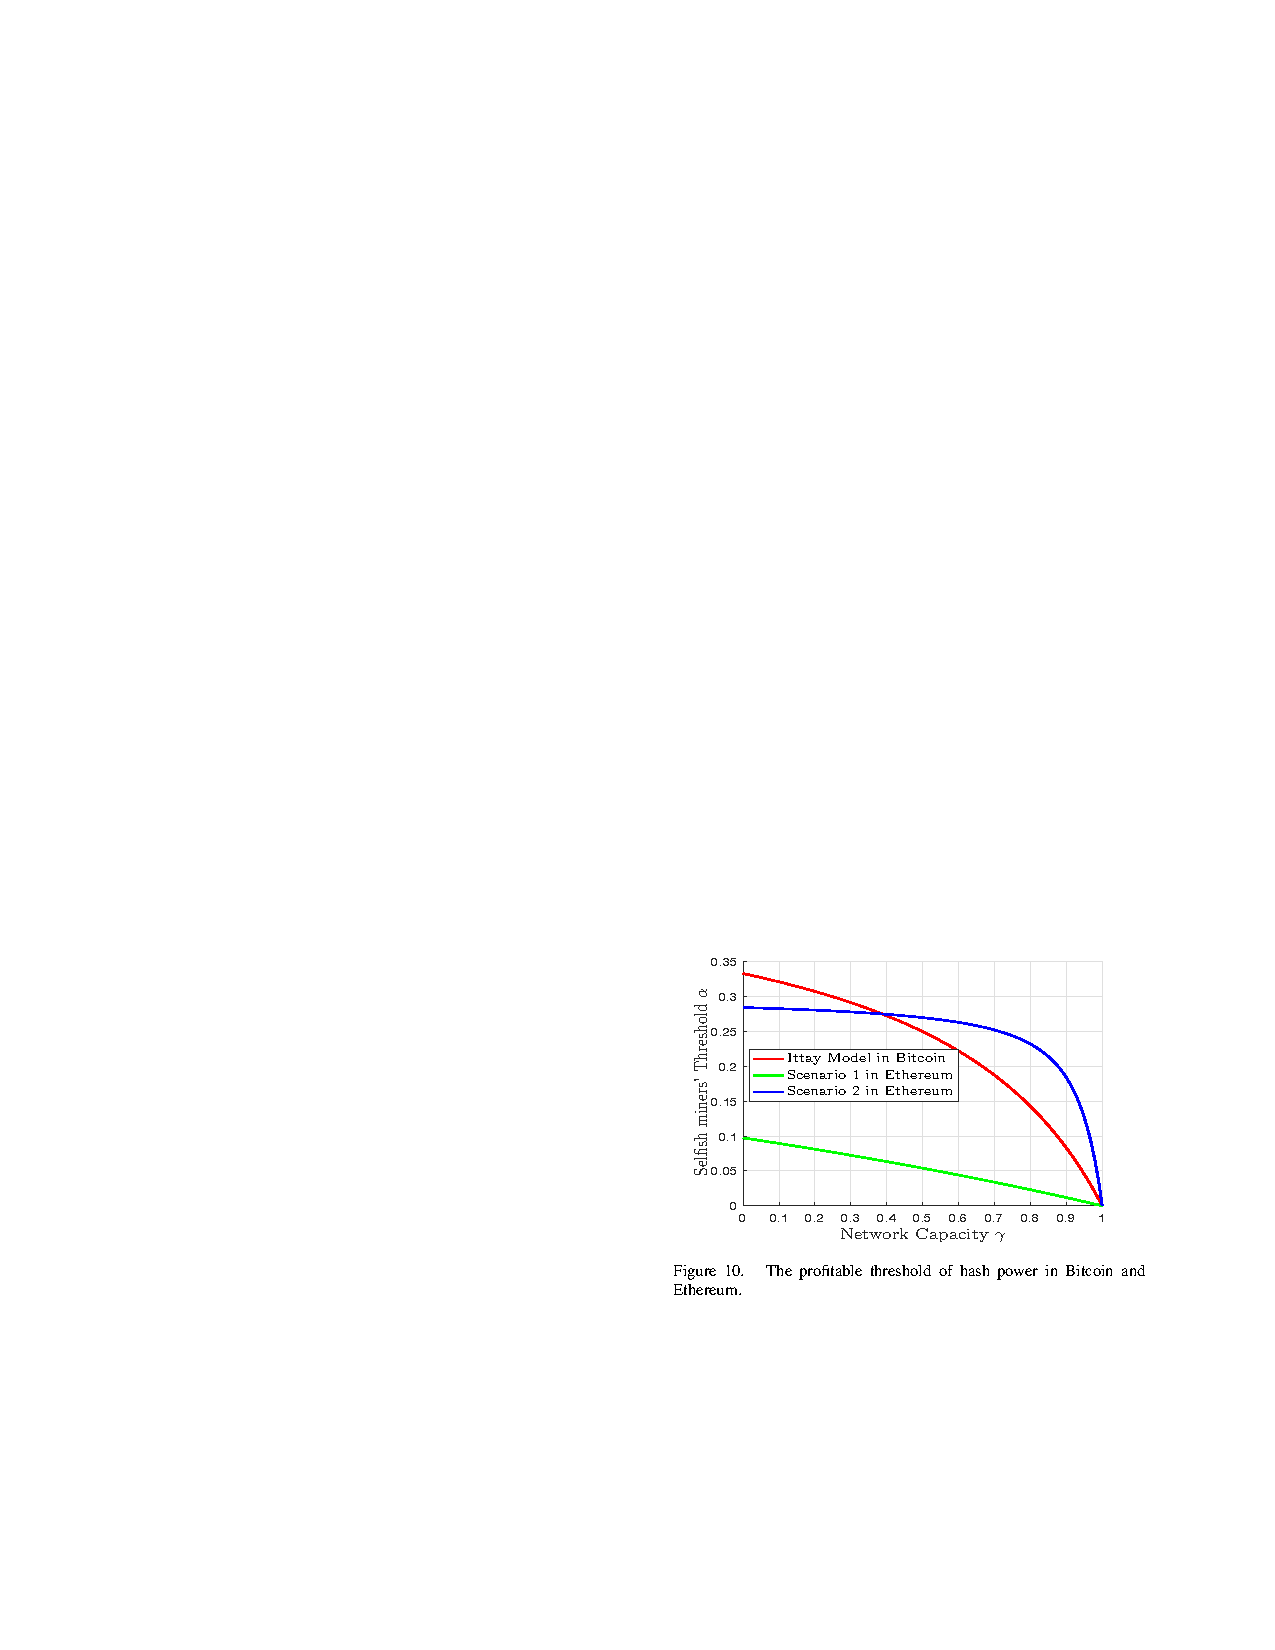
\includegraphics{fig/inclusive-selfish-mining}
	\end{figure}
	In the above figure from [Selfish Mining in Ethereum, ICDCS'19] Scenario 1 is where block difficulty is only adjusted based on the new blocks on the main chain.
	Scenario 2 adjusts difficulty based on creation of blocks and uncle blocks.
	
\end{proof}

\section{Uncles for scaling}
In Ethereum, the transactions included in uncle blocks are not applied. However, it is possible to also apply these transactions.

\begin{theorem}
	\label{thm:uncleorder}
It is possible to define a deterministic order on all blocks in a chain and all uncles in a chain, such that the order extends when the chain is extended.
This allows to execute transactions that are included in the uncle blocks, but not in the main chain.
\end{theorem}

\begin{proof}
	The order is done based on the following principles, from highest to lowest priority:
	\begin{itemize}
		\item Ancestors of $b_{new}$ are ordered before uncles of $b_{new}$.
		\item Uncles of $b_{new}$ are ordered before $b_{new}$.
		\item Uncles are ordered according to their depth.
		\item At the same depth, uncles are ordered according to their hash.
	\end{itemize}
\end{proof}

\begin{note}
Inclusive blockchains have the following effect on scalability:
\begin{itemize}
	\item If uncle blocks include transactions that are not included or conflicting with the main chain this can further increase scalability. Execution of transaction in uncles is not implemented in Ethereum.
	\item Given execution of transactions in uncles, it is difficult how to incentivize different blocks in a fork, to include different transactions.
	\item It is possible to extend inclusive blockchains to allow uncles that are not children of ancestors in the current main chain. Theorem~\ref{thm:uncleorder} still holds, but becomes more complex.
\end{itemize}
\end{note}

\section{Bitcoin NG}
See resources.md on course info for Video, slides, paper, ...

\begin{definition} Bitcoin-NG differentiates between \emph{Keyblocks} and \emph{Microblocks}. 
	\begin{description}
		\item[Keyblocks] Include a proof of work. No transactions, a public key, and the hash of the last Key- or Microblock.
		\item[Microblocks] Include no PoW but transactions, a previous block hash, and a signature matching public key from last KeyBlock.
	\end{description}

	\noindent
	\textbf{Fork resolutions} Longest chain rule (or GHOST) is used but only looks at the Keyblocks.
	\textbf{Fee distribution} Fees are distribution between the creator of the microblock (40\%) and the creator of the next Keyblock (60\%).
\end{definition}

\begin{note} 
	(Bitcoin-NG)\newline
	
	
	\begin{itemize}
		\item Security and fork probability (keyblocks) is decoupled from throughput and transaction rate (microblocks).
		\item The distribution of fees (40/60) ensures that it is better to reference the latest microblock, rather than keeping the transactions for your own microblocks. Also significant incentive for actually publishing microblocks.
	\end{itemize}

\noindent	
\textbf{Problem}
	\begin{itemize}
		\item Since Bitcoin-NG relies on a leader, progress can be reduced through leader failure. A single leader failure will not be a problem, but if an attacker causes multiple leaders to fail, e.g. by a DDOS (Distributed denial of service) attack, transaction throughput may be significantly reduced.
	\end{itemize}
\end{note}

\begin{example}
To understand the choice of 40\%, 60\% fee distribution, consider the example in Figure~\ref{fig:bitng-1}. Squares represent key blocks, while circles represent microblocks. 

In Figure~\ref{fig:bitng-1} the minor of the red block gets 60\% of the fees from the yellow transactions from microblock $b_0'$.

If he instead mines on top of $b_0$, he can himself publish a microblock including the yellow transactions. This is shown in Figure~\ref{fig:bitng-2}.
In this case the red minor receives 40\% of the fees from yellow transactions. 
Additionally, if the red minor has a fraction of the mining power equal to $\alpha$, he has a probability $\alpha$ to mine key-block $b_2$ and get additional 60\% of the yellow fees. 
If $\alpha<0.33$ then $0.4+\alpha\cdot 0.6 < 0.6$. Thus the red minor will try to extend $b_0'$.

Similarly, if the blue minor does not publish block $b_0'$ but instead hopes to publish $b_2$ in Figure~\ref{fig:bitng-2}, his expected fraction of the yellow fees is $\beta\cdot 0.6 <0.4$. Thus for a hashing fraction $\beta<0.33$ it is better to publish $b_0'$.
	\begin{figure}[h]
		\centering
		%!TEX root = ../main.tex

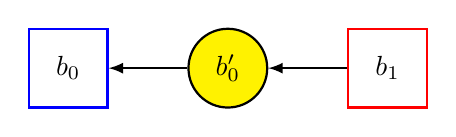
\begin{tikzpicture}
	[block/.style={rectangle,draw,thick, minimum size=1cm},
	mblock/.style={circle,draw,thick, minimum size=1cm},
	dblock/.style={block, dashed},
	noblock/.style={block, white},
	prev/.style={draw, -latex, thick}, 
	dprev/.style={prev, dashed},
	just/.style={-latex, double, thick, red},
	justarc/.style={out=135, in=45},
	interval/.style={|-|, dashed, thick},
	node distance =.5cm and 1cm]
	\node(b0)[block, draw=blue]{$b_0$};
	\node(b1)[mblock, right=of b0, fill=yellow]{$b_0'$};
	\draw[prev](b1) -- (b0);
	\node(b2)[block, right=of b1, draw=red]{$b_1$};
	\draw[prev](b2) -- (b1);
	
	
	
\end{tikzpicture}
		\caption{Red miner gets 60\% of yellow transactions.}
		\label{fig:bitng-1}
	\end{figure}
	\begin{figure}[h]
		\centering
		%!TEX root = ../main.tex

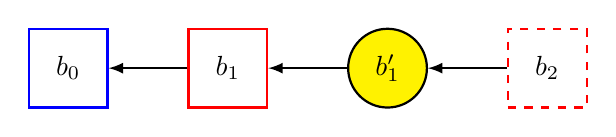
\begin{tikzpicture}
	[block/.style={rectangle,draw,thick, minimum size=1cm},
	mblock/.style={circle,draw,thick, minimum size=1cm},
	dblock/.style={block, dashed},
	noblock/.style={block, white},
	prev/.style={draw, -latex, thick}, 
	dprev/.style={prev, dashed},
	just/.style={-latex, double, thick, red},
	justarc/.style={out=135, in=45},
	interval/.style={|-|, dashed, thick},
	node distance =.5cm and 1cm]
	\node(b0)[block,draw=blue]{$b_0$};
	\node(b1)[block, right=of b0, draw=red]{$b_1$};
	\draw[prev](b1) -- (b0);
	\node(b2)[mblock, right=of b1, fill=yellow]{$b_1'$};
	\draw[prev](b2) -- (b1);
	\node(b3)[dblock, right=of b2,draw=red]{$b_2$};
	\draw[prev](b3) -- (b2);
	
	
	
\end{tikzpicture}
		\caption{Red miner expects to get $40+\alpha\cdot 60$\% of the yellow transactions.}
		\label{fig:bitng-2}
	\end{figure}

	
\end{example}



\section{Sharding for blockchains}
When sharding, the idea is to divide the blockchain into many smaller chains. Each small chain (i.e. shard) maintains part of the data.

\begin{definition} In a \emph{sharded blockchain} every node only maintains a part of the data and processes transactions that access the data he stores.
\end{definition}

\begin{note} \textbf{Problems for sharding:}
	\begin{enumerate}[label=\Alph*)]
		\item How to distribute the state?
		\item How to process updates that access state in multiple shards?
		\item How to avoid that an attacker takes over one shard?
	\end{enumerate}
\noindent
\textbf{Solutions}
\begin{enumerate}[label=\Alph*)]
	\item Using consistent hashing. E.g., shard 1 stores all outputs that belong to addresses that start with 01.
	\item There are different cases:
	\begin{itemize}
		\item Payments from one shard to another, can be split into a withdrawal and deposit. Execute withdrawal first. To execute deposit, must reference withdrawal.
		\item Transactions that are conditioned on multiple shards use a variant of 2 Phase Commit, e.g. first lock required outputs. When all necessary outputs are locked, execute transaction.
	\end{itemize}
	Note that variant 2 can diminish the benefit of sharding, since it requires coordination and locks state.
	\item There are two ideas:
	\begin{itemize}
		\item Distribute miners to shards according to their hashes, and redistributed frequently.
		\item Allow miners to participate in multiple shards, and to publish blocks on multiple shards with a single proof of work. 
		
	\end{itemize}
	Both of these are problematic. In the first, redistribution is reducing the benefit of sharding. The second encourages miners to form pools.
\end{enumerate}

\end{note}

\chapter{System models}
%!TEX root = ../main.tex

\noindent
In the Bitcoin protocol, any node can join. Additional any entity can create multiple accounts on bitcoin. Accounts are per default anonymous.
This model is called \textbf{unpermissioned}. No permission is needed to participate. 

\section{Unpermissioned systems}
In an unpermissioned system anyone can join, usually anonymity is provided.
Thus the creation of sybils is usually possible.

To mitigate the existence of sybils, unpermissioned blockchains use Proof of Work or Proof of Stake or similar mechanisms.

\section{Permissioned systems}
Permissioned systems assume there exists a list of members.
New members need permission or authentication via a central authority to join. 
Table~\ref{tab:members} gives an example of a table of members.. Typically assume that all members have a copy of the membership list. 

The existence of a membership list, or possibility to create and distribute one
is often referred to as public key infrastructure (PKI).
It allows any two members to contact each other (using listed IP addresses), and create an authenticated channel (using public keys).

\begin{table}[h]
	\centering
	\begin{tabular}{| c | c | c | c | }
		\hline
		ID & $pubkey$ & IP & ... \\
		\hline
		1 & 0x1f3 & &\\
		\hline
		2 & 21xf3 & &\\
		\hline
		
	\end{tabular}
	\caption{Membership list example. \label{tab:members}}
\end{table}

In a permissioned system the central authority prevents sybils.

\begin{example}
	\begin{enumerate}
		\item The classical example for a permissioned blockchain is a blockchain run together by a set or organizations. Typically we assume that each organization runs a node. The libra blockchain is an example for this. For libra, a non-profit central organization exists, which is functioning as central authority.
		\item If a single system, run within one organization is running on multiple servers, this also is a permissioned system. The different servers have unique ids and the system administrator functions as central authority.
		\item A more open example is a system that requires nodes to authenticate with Bank-ID, passport or sharing their social media activity. 
		Here the central authority is the issuer of Bank-ID, passport or social media.
	\end{enumerate}
\end{example}


\section{Failure models}
We distinguish different failure models, based on the failure assumptions, e.g. what failures may happen.
All apply to permissioned systems, some are applicable to unpermissioned systems.

\paragraph{No failure}
Assuming that members do not fail, it is possible to use authenticated channels for trusted interactions.

\paragraph{Central node does not fail}
Given a centralized node, that processes trust to not fail, they can build a centralized system, where the trusted node is responsible to manage state and interaction for the other members.

This model is used in cloud services, where all users connect to the service provider and trust this provider to store and maintain their application state and coordinate interactions with other users.

\paragraph{Crash failure}
In this model, nodes can stop by crash failures. It is not possible to communicate with a crashed node and the data stored on a crashed node may be lost.

This model is often assumed for machines that cooperatively run a service within a trusted domain, e.g. servers within a data center. 

In this model it is possible to implement consistent services, e.g. a blockchain, that work as long as a majority of the nodes is running. Examples are the Paxos algorithm thaught in DAT520.

In this model, as shown by the Paxos algorithm it is possible to develop systems that simply halt, when the failure threshold is violated.
Thus, even if a majority of nodes fail, nothing bad will happen.

\paragraph{Byzantine fault tolerance BFT}
It is assumed that \emph{any node may fail or misbehave}, i.e. a faulty node may not only stop, but may act maliciously, trying to sabotage the application. However, it is assumed that \emph{only a small fraction of the nodes actually fail or misbehave}.

Misbehavior may for example be caused by 
\begin{itemize}
	\item virus or malware
	\item misconfiguration
	\item sabotage
\end{itemize}
The above assumption says, that at most a small fraction of the nodes will be victim to any of these.

In this model it is possible to implement consistent services, e.g. a blockchain, that works as long as a large majority, e.g. 2/3 of the members are correct.

\paragraph{Selfish or rational misbehavior}
All nodes could misbehave if it benefits them. Such nodes are called \emph{selfish} or \emph{rational}.
Different from the BFT model, we do not assume a failure threshold, but we assume, nodes will not misbehave if this is not in their interest.

In this model it is possible to design algorithms using game theory. 
For this, every node is assigned a utility function:

For example the utility of participating in bitcoin mining is the block reward and transaction fees, minus costs for computation and networking, e.g. energy and hardware.

The goal for game theory is to show that nodes cannot increase their utility, by deviating from a protocol, e.g. by deviating from the longest chain rule.

\chapter{A BFT blockchain protocol}
	\label{ch:BFT}
	\section{Proof of certification}
	\label{sec:poc}
	%!TEX root = ../main.tex

\noindent
Unpermissioned blockchains require that published blocks carry a nonce that causes the block hash to be meet a specific difficulty (e.g. start with a specific number of zeros). The this proof of work has two main functionalities:

\begin{enumerate}
	\item \textbf{Publishing rate:} Requiring a proof of work ensures that blocks are published at a limited rate. This ensures that, whp., a block is propagated throughout the network, before the next block is published.
	\item \textbf{Fork probability:} If, while a block is propagated throughout the network, another block is published, these blocks create a fork and put the system in an undecided state. Proof of work ensures that the probability that two blocks are found concurrently is small. 
\end{enumerate}

In a permissioned system, similar guarantees can be achieved using a certificate.

\begin{definition}[System Model]
	A permissioned system is comprised of $N$ nodes $n_1, n_2, ..., n_N$.
	We assume that nodes have access to digital signatures, and that each node knows public keys of all other nodes.	
\end{definition}

\begin{definition}
A certificate for a block $b$ is a collection of digital signatures for $b$. 
A certificate contains signatures from more than $N\cdot\frac{2}{3}$ different nodes. We write $c_{min}$ for the minimum number of signatures contained in a certificate $$c_{min} = \left\lceil\frac{2N+1}{3}\right\rceil$$
\end{definition}


\begin{idea} We now give an intuition how certificates can limit publishing rate and fork probability:
	\begin{enumerate}
		\item \textbf{Publishing rate:} To publish a block with certificate, this block has to be transmitted, validated and signed by at least $c_{min}$ nodes. Thus, blocks cannot be published faster, than (most) of the nodes can validate them.
		\item \textbf{Fork probability:} If less than $\frac{N}{3}$ nodes signed multiple conflicting blocks, no two conflicting blocks can both receive a certificate.
	\end{enumerate}
\end{idea}

	
	\section{Safety}
	\label{sec:safe1}
	%!TEX root = ../main.tex

\noindent
In the following we define a set of rules that correct nodes should follow. We assume that at least $c_{min}$ nodes are following these rules.

\begin{figure}
	\centering
	%!TEX root = ../main.tex

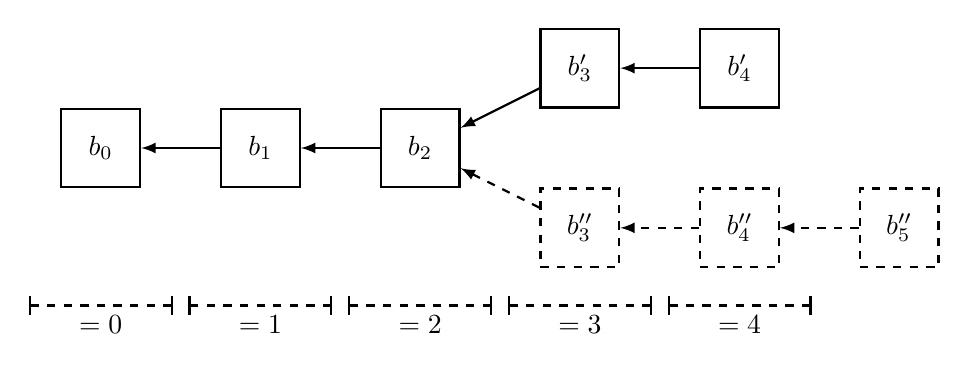
\begin{tikzpicture}
	[block/.style={rectangle,draw,thick, minimum size=1cm},
	dblock/.style={block, dashed},
	noblock/.style={block, white},
	prev/.style={draw, -latex, thick}, 
	dprev/.style={prev, dashed}, 
	interval/.style={|-|, dashed, thick},
	node distance =.5cm and 1cm]
	\node(b0)[block]{$b_0$};
	\node(b1)[block, right=of b0]{$b_1$};
	\draw[prev](b1) -- (b0);
	\node(b2)[block, right=of b1]{$b_2$};
	\draw[prev](b2) -- (b1);
	\node(b3)[noblock, right=of b2]{};
	\node(b3a)[block, above right=of b2.east]{$b_3'$};
	\draw[prev](b3a) -- (b2);

	\node(b3b)[dblock, below right=of b2.east]{$b_3''$};
	\draw[dprev](b3b) -- (b2);
	
	\node(b4)[noblock, right=of b3]{};
	\node(b4b)[dblock, right=of b3b.east]{$b_4''$};
	\draw[dprev](b4b) -- (b3b);
	\node(b4a)[block, right=of b3a.east]{$b_4'$};
	\draw[prev](b4a) -- (b3a);

	\node(b5)[noblock, right=of b4]{};
	\node(b5b)[dblock, right=of b4b.east]{$b_5''$};
	\draw[dprev](b5b) -- (b4b);
	
	
	
	\foreach \x in {0, 1, 2,3,4}{
	\draw[interval] ([xshift=-.4cm,yshift=-2cm]b\x.west) -- node[below]{$\depth=\x$} ([xshift=.4cm,yshift=-2cm]b\x.east);};
	
\end{tikzpicture}
\caption{Blocks in a tree and depth $d$ of blocks.}
\label{fig:tree}
\end{figure}

The \emph{previousBlock} pointers create a tree structure on blocks. We can thus refer to the \emph{depth} of a block. We write $b.\depth$ for the depth of block $b$. Figure~\ref{fig:tree} shows a tree with different depth levels. Here $b_4''.\depth=4$. Similarly, we refer to the parent, ancestors or descendants of a block. In Figure~\ref{fig:tree}, e.g., $b_5''$ is a descendant of $b_3''$ and all blocks are descendants of $b_0$. Further, $b_3'$ is the parent of $b_4'$ and $b_2$ is an ancestor of $b_4'$. 

We can not define the first rule.
\begin{Rule}
After signing a block at depth $d$, only sign at depth $d'>d$.
\end{Rule}
\noindent
The first rule says that nodes should only sign at increasing depth. Especially, they should not sign at the same depth twice.

As noted in Section~\ref{sec:poc}, to prevent forks we should also add a rule that prohibits changing from one branch of the tree to another, e.g., signing  $b_5''$ in Figure~\ref{fig:tree} after signing $b_3'$ and $b_4'$.
%
We further note, that it is possible, that no block at a certain depth receives a certificate. E.g.,~$b_3'$ and $b_3''$ may both be signed by 5 out of 10 nodes. Thus, no block has the required ($c_{min}(10)=7$) signatures.  
%
Therefore it should still be allowed for a node to sign $b_4'$ after signing $b_3''$. 
%

\begin{definition}The \emph{locked block} at node $n_i$, $n_i.\lock$ is the block $b$ at highest depth, such that $n_i$ has (or has seen) a certificate for $b$.
\end{definition}

\begin{Rule} 
	A node $n_i$ only signs a block that is a descendant of $n_i.\lock$.	
\end{Rule}

We note that if $c_{min}$ nodes sign a block $b$, that does not imply that these nodes know the certificate of this block. Certificates have to be collected and disseminated by some node. We therefore define the following:

\begin{definition} We assume that every block $b_i$ contains a certificate for a block $b_j$ such that $b_j$ is an ancestor of $b_i$. We say that $b_i.\just=b_j$. 	
\end{definition}

\begin{lem}
	For some node $n_i$ that follows Rule 2, it holds that, after signing block $b$, $n_i.\lock.\depth\geq b.\just.\depth$ holds.
\end{lem}

\begin{example} In Figure~\ref{fig:tree}, if $b_4'.\just=b_3'$, then after signing $b_4'$ a node following Rule~2 will not sign $b_5''$.	
\end{example}

\begin{figure}
	\centering
	%!TEX root = ../main.tex

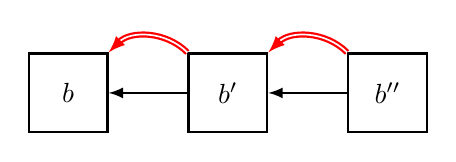
\begin{tikzpicture}
	[block/.style={rectangle,draw,thick, minimum size=1cm},
	dblock/.style={block, dashed},
	noblock/.style={block, white},
	prev/.style={draw, -latex, thick}, 
	dprev/.style={prev, dashed},
	just/.style={-latex, double, thick, red},
	justarc/.style={out=135, in=45},
	interval/.style={|-|, dashed, thick},
	node distance =.5cm and 1cm]
	\node(b0)[block]{$b$};
	\node(b1)[block, right=of b0]{$b'$};
	\draw[prev](b1) -- (b0);
	\node(b2)[block, right=of b1]{$b''$};
	\draw[prev](b2) -- (b1);
	
	
	\foreach \from/\to in {b1/b0, b2/b1}{
		\draw[just] (\from) to[justarc] (\to);
	}
	
\end{tikzpicture}
	\caption{Blockes with red justification link, confirm block $b$.}
\end{figure}

\begin{definition}
\label{def:confirmed}	
We say that a block $b$ is \emph{confirmed}, if there exist blocks $b'$ and $b''$, such that, $b=b'.\just$, $b'=b''.\just$, and $b.\depth = b''.\depth-2$.	
\end{definition}

We note that the notion of a confirmed block is similar to proof of work blockchains like bitcoin, where a block counts as confirmed if it has been extended by a certain number of blocks, e.g. 6 blocks in bitcoin.

\begin{theorem}\label{thm:confirmed}
If nodes follow Rule~2 and a block $b$ is confirmed, then any certified block at depth $d>b.\depth$ is a descendant of $b$.
\end{theorem}

\begin{proof}
If $b$ is confirmed, there exist $b'$ and $b''$ as in Definition~\ref{def:confirmed}. $b''$ contains a certificate for $b'$. Thus at least $c_{min}$ nodes have signed $b'$. $b'$ contains a certificate for $b$. Thus upon signing $b'$, a node $n_i$ sets $n_i.\lock=b$.

We have to show that every certified block $\beta$ with $\beta.\depth > b.\depth$ is a descendant of $b$. We proof this by induction over $\Delta_d=\beta.\depth-b.\depth$. 

If $\Delta_d=1$ then $\beta=b'$ since at most one block at depth $b.\depth+1$ can be certified. 

Let $\Delta_d=n+1$. Both $\beta$ and $b'$ are signed by $c_{min}$ nodes. 
Let $n_i$ be a correct nodes (following Rules~1 and~2) that signed both $\beta$ and $b'$. Due to Rule~1,  $n_i$ signed $b'$ before $\beta$. 
Thus $n_i.\lock=b$ did hold. The induction hypothesis implies that when signing $\beta$, $n_i.\lock$ was either $b$ or a descendant of $b$. Rule~2 implies that $\beta$ is a descendant of $n_i.\lock$. Thus $\beta$ is a descendant of $b$.
\end{proof}
	
	\section{Liveness}
	\label{sec:live}
	%!TEX root = ../main.tex

\noindent
In Section~\ref{sec:safe1} we have defined rules, how correct nodes should sign blocks and how we can identify confirmed blocks, based on published blocks.

However, we did not define when and how blocks should be created. Further, we note that if at every depth, many blocks are created, it is possible that no block will ever receive a certificate.

To resolve this, we assign leaders to every depth and only allow the leader to publish blocks at his depth:
\[
\textrm{leader}(\depth)=n_{\depth\ \text{mod} N}
\]

Algorithm~\ref{alg:leader} shows how nodes only sign blocks at the next depth and only if the block is published by $\textrm{leader}(\depth)$.
However, based on a timeout, nodes can hop over one depth.

\begin{algorithm}
	\caption{Rotating leader}
	\label{alg:leader}
	\begin{algorithmic}[1]
		\State{$\depth=1$}
		\State{$timer=\text{start}()$}
		\On{receive $b$ from $\textrm{leader}(\depth)$}
			\If{$b.\just.\depth > \lock.\depth$}
				\State{$\lock=b.\just$}
			\EndIf
			\If{$b.\depth=\depth$ and $b$ descendant of \lock}
				\State{$\text{sign}(b)$}
				\State{$\depth++$}
				\State{$timer=\text{restart}()$}
			\EndIf
		\EOn
		\On{$timer$ finish}
			\State{$\depth++$}
			\State{$timer=\text{restart}()$}
		\EOn
		\On{$\textrm{leader}(\depth)=self$}\label{line:leader}
			\State{ask all nodes for locked certificate}
			\label{line:wait}
			\If{block is missing ad depth $\depth-1$}
				\State{create empty block at $\depth-1$}
			\EndIf
			\State{create block at $\depth$ including deepest certificate}
			\label{line:leaderend}
		\EOn
	\end{algorithmic}
\end{algorithm}	

Lines~\ref{line:leader} to~\ref{line:leaderend} show how a correct node should propose a block. 
First a correct node needs to query other nodes, especially his predecessor, for certificates they have collected.
There are two cases:
\begin{enumerate}[label=\alph*)]
	\item If a nodes collects a certificate for the last block $(\depth-1)$, he can immediately publish a new block including this certificate.
	\item\label{case:notlast} If a nodes does only collect certificates for older blocks. He includes the certificate at highest depth in his block. If no block at $\depth-1$ is known to the node, he may also create that block.
\end{enumerate}
The situation from Case~\ref{case:notlast} is also shown in Figure~\ref{fig:newblock}.

\begin{figure}[h!]
	\centering
	%!TEX root = ../main.tex

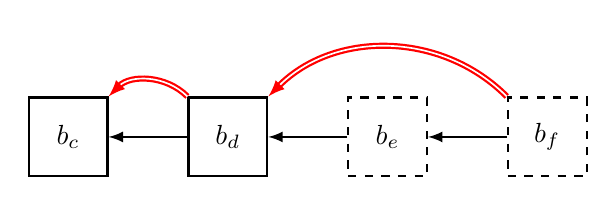
\begin{tikzpicture}
	[block/.style={rectangle,draw,thick, minimum size=1cm},
	dblock/.style={block, dashed},
	noblock/.style={block, white},
	prev/.style={draw, -latex, thick}, 
	dprev/.style={prev, dashed},
	just/.style={-latex, double, thick, red},
	justarc/.style={out=135, in=45},
	interval/.style={|-|, dashed, thick},
	node distance =.5cm and 1cm]
	\node(b0)[block]{$b_c$};
	\node(b1)[block, right=of b0]{$b_d$};
	\draw[prev](b1) -- (b0);
	\node(b2)[dblock, right=of b1]{$b_e$};
	\draw[prev](b2) -- (b1);
	\node(b3)[dblock, right=of b2]{$b_f$};
	\draw[prev](b3) -- (b2);
	
	
	
	\foreach \from/\to in {b1/b0,b3/b1}{
		\draw[just] (\from) to[justarc] (\to);
	}
	
\end{tikzpicture}
	\caption{Leader for $b_f.\depth$ may also create $b_e$.}
	\label{fig:newblock}
\end{figure}
	
\begin{figure}[h!]
	\centering
	%!TEX root = ../main.tex

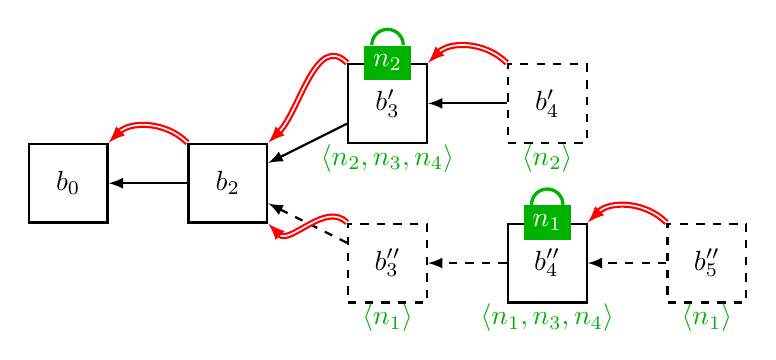
\begin{tikzpicture}
	[block/.style={rectangle,draw,thick, minimum size=1cm},
	dblock/.style={block, dashed},
	noblock/.style={block, white},
	prev/.style={draw, -latex, thick}, 
	dprev/.style={prev, dashed}, 
	just/.style={-latex, double, thick, red},
	justarc/.style={out=135, in=45},
	interval/.style={|-|, dashed, thick},
	sign/.style={green!70!black, fill=white},
	node distance =.5cm and 1cm]
	\node(b0)[block]{$b_0$};
	
	\node(b2)[block, right=of b0]{$b_2$};
	\draw[prev](b2) -- (b0);
	\node(b3)[noblock, right=of b2]{};
	\node(b3a)[block, above right=of b2.east]{$b_3'$};
	\draw[prev](b3a) -- (b2);

	\node(b3b)[dblock, below right=of b2.east]{$b_3''$};
	\draw[dprev](b3b) -- (b2);
	
	\node(b4)[noblock, right=of b3]{};
	\node(b4b)[block, right=of b3b.east]{$b_4''$};
	\draw[dprev](b4b) -- (b3b);
	\node(b4a)[dblock, right=of b3a.east]{$b_4'$};
	\draw[prev](b4a) -- (b3a);

	\node(b5)[noblock, right=of b4]{};
	\node(b5b)[dblock, right=of b4b.east]{$b_5''$};
	\draw[dprev](b5b) -- (b4b);

	\foreach \from/\to in {b2/b0, b3a/b2, b4a/b3a, b5b/b4b}{
		\draw[just] (\from) to[justarc] (\to);
	}
	\draw[just] (b3b) to[justarc, in=315] (b2);
	% \draw[just] (b5b) to[justarc, in=0] (b2);
	
	\node at (b3a.south)[below=0, inner sep=0,sign]{$\langle n_2,n_3, n_4\rangle$};
	\node at (b3b.south)[below=0, inner sep=0,sign]{$\langle n_1\rangle$};
	\node at (b4a.south)[below=0, inner sep=0,sign]{$\langle n_2\rangle$};
	\node at (b4b.south)[below=0, inner sep=0,sign]{$\langle n_1,n_3, n_4\rangle$};
	\node at (b5b.south)[below=0, inner sep=0,sign]{$\langle n_1\rangle$};
	
	\node (l2) at (b3a.north) [white,rectangle, fill=green!70!black]{$n_2$};
	\draw [green!70!black, very thick] ([xshift=2mm]l2.north) arc [start angle = 0, end angle=180, radius=2mm];
	\node (l1) at (b4b.north) [white,rectangle, fill=green!70!black]{$n_1$};
	\draw [green!70!black, very thick] ([xshift=2mm]l1.north) arc [start angle = 0, end angle=180, radius=2mm];
	
\end{tikzpicture}
	\caption{Figure illustrating Example~\ref{ex:problem1}.}
	\label{fig:problem}
\end{figure}

\begin{example}\label{ex:problem1}
Assume $N=4$. Thus $c_{min}=3$ and we have nodes $n_1$, $n_2$, $n_3$, and $n_4$.

In Figure~\ref{fig:problem}, green subscript shows the nodes that have signed a specific block. Nodes $n_2$, $n_3$, and $n_4$ have signed $b_3'$, while $n_1$ has signed $b_3''$. Further, $n_2$ has signed $b_4'$. Thus $n_2.\lock=b_3'$. We assume that only $n_2$ has seen the certificate for $b_3'$.

Since $n_3$ and $n_4$ have not seen a certificate for $b_3'$ they have, together with $n_1$ signed $b_4''$. $n_1$ has seen this certificate, when signing $b_5''$. Thus $n_1.\lock=b_4''$. We note that in this example, none of the nodes have behaved faulty.
\end{example}	


\begin{example}\label{ex:problem}
This example extends Example~\ref{ex:problem1}. Thus we again assume $N=4$.
In Figure~\ref{fig:problem} shows a situation as in Example~\ref{ex:problem1}.

Node $n_2$ has locked $b_3'$ and node $n_1$ has locked $b_4''$.
We note that Rule~2 prohibits $n_2$ from signing $b_6''$ and $n_1$ from signing $b_6'$. This may deadlock the system. 

However we note that Rule~2 allows $n_2$ to sign $b_5''$ as shown in Figure~\ref{fig:problem1}. The reason is that $b_5''$ includes a certificate for $b_4''$. This allows $n_2.\lock$ to be updated.
\end{example}

In Example~\ref{ex:problem}, it is not helpful, to let $n_1$, $n_3$ and $n_4$ report whether they have voted for $b_4'$ or $b_4''$. The reason for this is that one node may violate Rule~1. Thus $n_3$ or $n_4$ may also sign $b_4''$. 
\begin{figure}[h!]
	\centering
	%!TEX root = ../main.tex

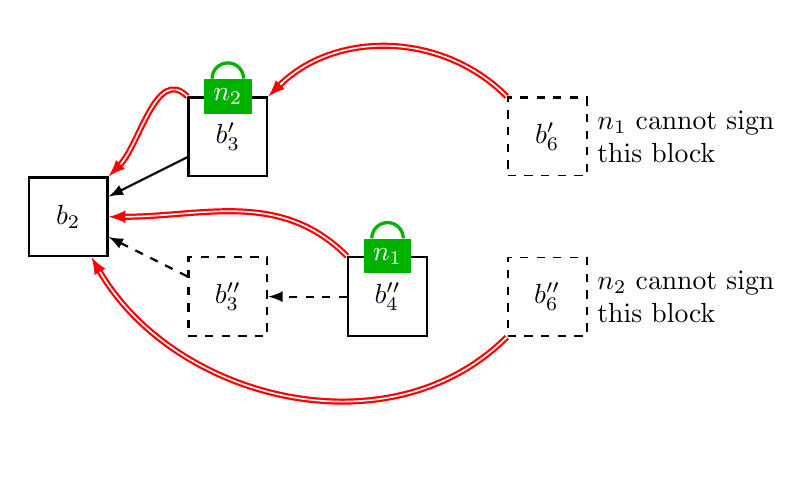
\begin{tikzpicture}
	[block/.style={rectangle,draw,thick, minimum size=1cm},
	dblock/.style={block, dashed},
	noblock/.style={block, white},
	prev/.style={draw, -latex, thick}, 
	dprev/.style={prev, dashed}, 
	just/.style={-latex, double, thick, red},
	justarc/.style={out=135, in=45},
	interval/.style={|-|, dashed, thick},
	sign/.style={green!70!black, fill=white},
	node distance =.5cm and 1cm]
	\node(b2)[block]{$b_2$};
	\node(b3)[noblock, right=of b2]{};
	\node(b3a)[block, above right=of b2.east]{$b_3'$};
	\draw[prev](b3a) -- (b2);
	\node(b4a)[noblock, right=of b3a.east]{$b_4'$};
	% \draw[prev](b4a) -- (b3a);
	\node(b5a)[dblock, right=of b4a.east]{$b_6'$};
	% \draw[prev](b5a) -- (b4a);
	

	\node(b3b)[dblock, below right=of b2.east]{$b_3''$};
	\draw[dprev](b3b) -- (b2);
	
	
	\node(b4)[noblock, right=of b3]{};
	\node(b4b)[block, right=of b3b.east]{$b_4''$};
	\draw[dprev](b4b) -- (b3b);
	\node(b5b)[dblock, right=of b4b.east]{$b_6''$};
	% \draw[](b5b) -- (b4b);

	\node(b5)[noblock, right=of b4]{};
	
	\foreach \from/\to in {b3a/b2, b5a/b3a}{
		\draw[just] (\from) to[justarc] (\to);
	}
	\draw[just] (b4b) to[justarc, in=0] (b2);
	\draw[just] (b5b) to[justarc, in=300, out=225] (b2);
	
	\node at (b5a.east) [right={0},align=left]{$n_1$ cannot sign\\ this block};
	\node at (b5b.east) [right={0},align=left]{$n_2$ cannot sign\\ this block};
	
	
	\node (l2) at (b3a.north) [white,rectangle, fill=green!70!black]{$n_2$};
	\draw [green!70!black, very thick] ([xshift=2mm]l2.north) arc [start angle = 0, end angle=180, radius=2mm];
	\node (l1) at (b4b.north) [white,rectangle, fill=green!70!black]{$n_1$};
	\draw [green!70!black, very thick] ([xshift=2mm]l1.north) arc [start angle = 0, end angle=180, radius=2mm];
	
\end{tikzpicture}
	\caption{Figure illustrating Example~\ref{ex:problem}.}
	\label{fig:problem}
\end{figure}	

Existing systems show two possible solutions for the problem shown in Example~\ref{ex:problem}. The PBFT algorithm allows $n_2$ to sign $b_6''$ if he receives messages from $n_1$, $n_3$ and $n_4$ saying that $b_2$ is their last certificate.

Other systems, like Tendermint, include a long timeout while collecting certificates on Line~\ref{line:wait}, during which the new leader waits for additional certificates. This ensures in Example~\ref{ex:problem}, if $n_1$ is correct, the certificate for $b_4''$ will be forwarded to the new leader.

	
	\section{Safety revisited}
	\label{sec:safe2}
	%!TEX root = ../main.tex

\noindent
In the following we present a variant of Rule~2 that does not lead to the problem from Example~\ref{ex:problem} in Section~\ref{sec:live}.

We first define a 3-locked block.
\begin{definition}
A node $n_i$ sets $n_i.\lock_3=b$, if $b$ is the block at highest depth, s.t. 
$n_i$ has signed a block $b''$ with $b''.\just=b'$ and $b'.\just=b$.
\end{definition}

\begin{figure}[h!]
	\centering
	%!TEX root = ../main.tex

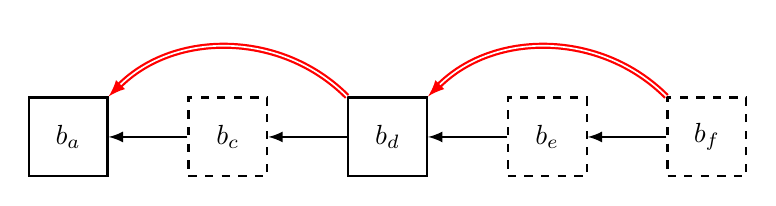
\begin{tikzpicture}
	[block/.style={rectangle,draw,thick, minimum size=1cm},
	dblock/.style={block, dashed},
	noblock/.style={block, white},
	prev/.style={draw, -latex, thick}, 
	dprev/.style={prev, dashed},
	just/.style={-latex, double, thick, red},
	justarc/.style={out=135, in=45},
	interval/.style={|-|, dashed, thick},
	node distance =.5cm and 1cm]
	
	\node(b0)[block]{$b_a$};
	\node(b1)[dblock, right=of b0]{$b_c$};
	\draw[prev](b1) -- (b0);
	\node(b2)[block, right=of b1]{$b_d$};
	\draw[prev](b2) -- (b1);
	\node(b3)[dblock, right=of b2]{$b_e$};
	\draw[prev](b3) -- (b2);
	\node(b4)[dblock, right=of b3]{$b_f$};
	\draw[prev](b4) -- (b3);
	
	
	
	\foreach \from/\to in {b2/b0,b4/b2}{
		\draw[just] (\from) to[justarc] (\to);
	}
	
\end{tikzpicture}
	\caption{Block $b_a$ is locked on signing $b_f$.}
	\label{fig:newlock}
\end{figure}

\begin{Rule}[replaces Rule~2]
	A node $n_i$ signs a block $b$ only if 
	\begin{enumerate}[label=\alph*)]
		\item $b$ is a descendant from $n_i.\lock_3$
		\item $b.\just.\depth>n_i.\lock_3.\depth$.  
	\end{enumerate}
\end{Rule}

\begin{figure}[h!]
	\centering
	%!TEX root = ../main.tex

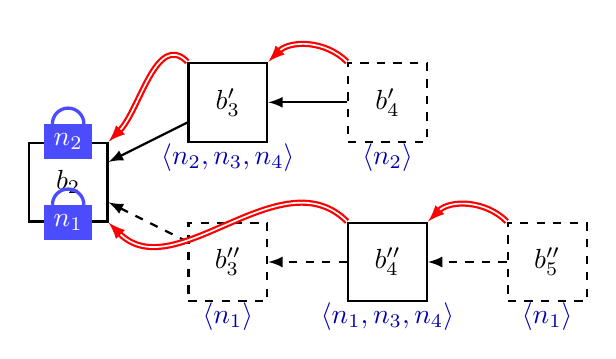
\begin{tikzpicture}
	[block/.style={rectangle,draw,thick, minimum size=1cm},
	dblock/.style={block, dashed},
	noblock/.style={block, white},
	prev/.style={draw, -latex, thick}, 
	dprev/.style={prev, dashed}, 
	just/.style={-latex, double, thick, red},
	justarc/.style={out=135, in=45},
	interval/.style={|-|, dashed, thick},
	sign/.style={blue!70!black, fill=white},
	node distance =.5cm and 1cm]
	
	\node(b2)[block]{$b_2$};
	\node(b3)[noblock, right=of b2]{};
	\node(b3a)[block, above right=of b2.east]{$b_3'$};
	\draw[prev](b3a) -- (b2);

	\node(b3b)[dblock, below right=of b2.east]{$b_3''$};
	\draw[dprev](b3b) -- (b2);
	
	\node(b4)[noblock, right=of b3]{};
	\node(b4b)[block, right=of b3b.east]{$b_4''$};
	\draw[dprev](b4b) -- (b3b);
	\node(b4a)[dblock, right=of b3a.east]{$b_4'$};
	\draw[prev](b4a) -- (b3a);

	\node(b5)[noblock, right=of b4]{};
	\node(b5b)[dblock, right=of b4b.east]{$b_5''$};
	\draw[dprev](b5b) -- (b4b);

	\foreach \from/\to in {b3a/b2, b4a/b3a, b5b/b4b}{
		\draw[just] (\from) to[justarc] (\to);
	}
	\draw[just] (b4b) to[justarc, in=315] (b2);
	% \draw[just] (b5b) to[justarc, in=0] (b2);
	
	\node at (b3a.south)[below=0, inner sep=0,sign]{$\langle n_2,n_3, n_4\rangle$};
	\node at (b3b.south)[below=0, inner sep=0,sign]{$\langle n_1\rangle$};
	\node at (b4a.south)[below=0, inner sep=0,sign]{$\langle n_2\rangle$};
	\node at (b4b.south)[below=0, inner sep=0,sign]{$\langle n_1,n_3, n_4\rangle$};
	\node at (b5b.south)[below=0, inner sep=0,sign]{$\langle n_1\rangle$};
	
	\node (l2) at (b2.north) [white,rectangle, fill=blue!70!white]{$n_2$};
	\draw [blue!70!white, very thick] ([xshift=2mm]l2.north) arc [start angle = 0, end angle=180, radius=2mm];
	\node (l1) at (b2.south) [white,rectangle, fill=blue!70!white]{$n_1$};
	\draw [blue!70!white, very thick] ([xshift=2mm]l1.north) arc [start angle = 0, end angle=180, radius=2mm];
	
\end{tikzpicture}
	\caption{Showing 3-locks that allow two sign any block extending $b_2$.}
	\label{fig:3locka}
\end{figure}

\begin{figure}[h!]
	\centering
	%!TEX root = ../main.tex

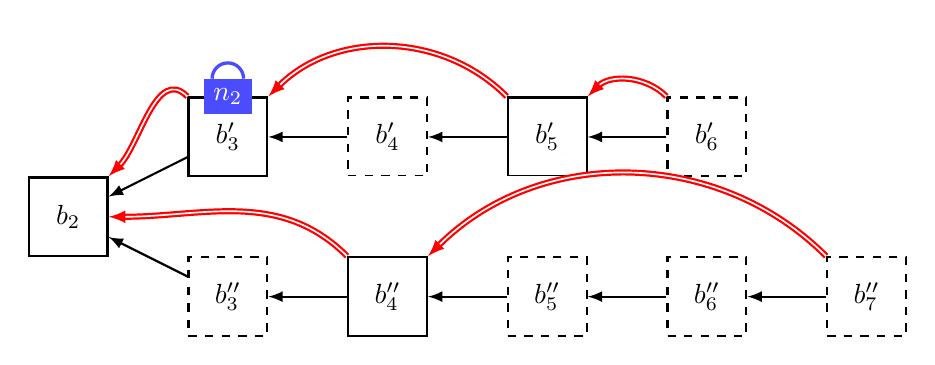
\begin{tikzpicture}
	[block/.style={rectangle,draw,thick, minimum size=1cm},
	dblock/.style={block, dashed},
	noblock/.style={block, white},
	prev/.style={draw, -latex, thick}, 
	dprev/.style={prev, dashed}, 
	just/.style={-latex, double, thick, red},
	justarc/.style={out=135, in=45},
	interval/.style={|-|, dashed, thick},
	sign/.style={blue!70!black, fill=white},
	node distance =.5cm and 1cm]
	
	\node(b2)[block]{$b_2$};
	\node(b3)[noblock, right=of b2]{};
	\node(b3a)[block, above right=of b2.east]{$b_3'$};
	\draw[prev](b3a) -- (b2);
	\node(b4a)[dblock, right=of b3a.east]{$b_4'$};
	\draw[prev](b4a) -- (b3a);
	\node(b5a)[block, right=of b4a.east]{$b_5'$};
	\draw[prev](b5a) -- (b4a);
	\node(b6a)[dblock, right=of b5a.east]{$b_6'$};
	\draw[prev](b6a) -- (b5a);


	\node(b3b)[dblock, below right=of b2.east]{$b_3''$};
	\draw[prev](b3b) -- (b2);
	
	\node(b4)[noblock, right=of b3]{};
	\node(b4b)[block, right=of b3b.east]{$b_4''$};
	\draw[prev](b4b) -- (b3b);
	
	\node(b5)[noblock, right=of b4]{};
	\node(b5b)[dblock, right=of b4b.east]{$b_5''$};
	\draw[prev](b5b) -- (b4b);
	\node(b6b)[dblock, right=of b5b.east]{$b_6''$};
	\draw[prev](b6b) -- (b5b);
	\node(b7b)[dblock, right=of b6b.east]{$b_7''$};
	\draw[prev](b7b) -- (b6b);

	\foreach \from/\to in {b3a/b2, b5a/b3a, b6a/b5a, b7b/b4b}{
		\draw[just] (\from) to[justarc] (\to);
	}
	\draw[just] (b4b) to[justarc, in=0] (b2);
	% \draw[just] (b5b) to[justarc, in=0] (b2);
	
	
	\node (l2) at (b3a.north) [white,rectangle, fill=blue!70!white]{$n_2$};
	\draw [blue!70!white, very thick] ([xshift=2mm]l2.north) arc [start angle = 0, end angle=180, radius=2mm];
	
	
\end{tikzpicture}
	\caption{Rule~3~b) allows $n_2$ to sign $b_7''$.}
	\label{fig:3lockb}
\end{figure}


\begin{example}
	Figure~\ref{fig:3locka} shows position of 3-locks in the same situation as shown in Figure~\ref{fig:problem1}. Rule~3  allows to sign any descendant of $b_2$.
	
Figure~\ref{fig:3lockb} shows a similar situation as in Figure~\ref{fig:problem}, only using 3-locks. $n_2$ has signed $b_6'$ and set its 3-lock to $b_3'$. The leader for depth 7 failed to collect the certificate for block $b_5'$ from $n_2$. Thus he extended block $b_4''$. 
Rule~2~b) still allows $n_2$ to sign $b_7''$.
\end{example}

Using Rule~3, it is enough if the leader waits for the last certificate from $c_{min}$ nodes on Line~\ref{line:wait} of Algorithm~\ref{alg:leader}.


\begin{definition}
\label{def:3confirmed}	
We say that a block $b$ is \emph{3-confirmed}, if there exist blocks $b'$, $b''$, and $\hat{b}$ such that, $b=b'.\just$, $b'=b''.\just$, and $b''=\hat{b}.\just$ 
and $b.\depth = b''.\depth-2$.	
\end{definition}

\begin{figure}
	\centering
	%!TEX root = ../main.tex

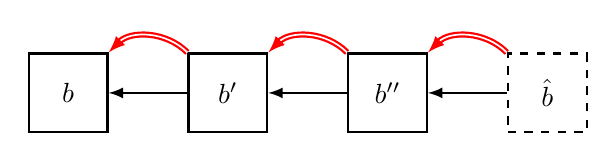
\begin{tikzpicture}
	[block/.style={rectangle,draw,thick, minimum size=1cm},
	dblock/.style={block, dashed},
	noblock/.style={block, white},
	prev/.style={draw, -latex, thick}, 
	dprev/.style={prev, dashed},
	just/.style={-latex, double, thick, red},
	justarc/.style={out=135, in=45},
	interval/.style={|-|, dashed, thick},
	node distance =.5cm and 1cm]
	\node(b0)[block]{$b$};
	\node(b1)[block, right=of b0]{$b'$};
	\draw[prev](b1) -- (b0);
	\node(b2)[block, right=of b1]{$b''$};
	\draw[prev](b2) -- (b1);
	\node(b3)[dblock, right=of b2]{$\hat{b}$};
	\draw[prev](b3) -- (b2);
	
	
	\foreach \from/\to in {b1/b0, b2/b1, b3/b2}{
		\draw[just] (\from) to[justarc] (\to);
	}
	
\end{tikzpicture}
	\caption{Block $b$ is 3-confirmed.}
\end{figure}

\begin{theorem}
If nodes follow Rule~3 (instead of Rule~2) and a block $b$ is 3-confirmed, then any certified block at depth $d>b.\depth$ is a descendant of $b$.
\end{theorem}

\begin{theorem}[Speculation]
Using Rule~3, if a node $n_i$ cannot sign a block $b$ due to Rule~3, then $n_i$ has a proof of misbehavior against the leader that published $b$.
\end{theorem}

\chapter{Smart Contracts}

	\section{Ethereum and Smart Contracts}
	See slides 

	\section{Smart Contract Security}
	See slides and \url{https://github.com/ethereumbook/ethereumbook/blob/develop/09smart-contracts-security.asciidoc}.
	
	\section{Oracles}
	
	\section{Off chain transactions}

\chapter{Hybrid blockchains}
	\label{ch:hybrid}
	%!TEX root = ../main.tex



\noindent
Blockchains like bitcoin, running in an unpermissioned setting only provide probabilistic guarantees. This applies both to proof of work, proof of stake or proof of utility based systems. This is different from BFT systems used in permissioned settings, that provide strong guarantees. 

\section{Consensus guarantees}
In this section we investigate the different guarantees given and techniques to build a hybrid system, providing strong guarantees in an unpermissioned setting.

\subsection{Bitcoin guarantees}
According to \href{https://www.usenix.org/system/files/conference/nsdi16/nsdi16-paper-eyal.pdf}{Bitcoin-NG}, the consensus mechanism deployed by Bitcoin (i.e. Nakamoto Consensus) gives the following guarantees assuming that Byzantine or misbehaving nodes hold at most $f<\frac{1}{4}$ of the mining power:

\begin{description}
	\item[Termination] There exists a time difference function $\Delta(\cdot)$ such that, given a time $t$ and a value $0<\epsilon<1$, the probability is smaller than $\epsilon$, that at times $t',t''>t+\Delta(\epsilon)$ a node returns two different states for the machine at time $t$.
	\item[Agreement] There exists a time difference function $\Delta(\cdot)$ such that, given a value $0<\epsilon<1$, the probability that at time $t$, two nodes return different states for $t-\Delta(\epsilon)$ is smaller than $\epsilon$.
	\item[Validity] If the fraction of mining power of Byzantine nodes is bounded by $f$, then the average fraction of state machine transitions that are not inputs of honest nodes is smaller than $f$.
\end{description}

Note especially that Termination and Agreement only hold probabilistically. 
This may not be a problem in practice, i.e., $\epsilon$ can be chosen small enough that the difference between probabilistic and absolute guarantees can be ignored. 
However, to achieve a small $\epsilon$ may require long waiting times, as in bitcoin where the confirmation of a block may take more than 1h.
Similarly, if one of these properties, e.g. Termination, is violated it is difficult to say wether this is due to the probabilistic nature of this property, or to the fact that assumptions on the failure threshold $f$ where violated.

\subsection{BFT guarantees}
In comparison, we now analyze agreement and termination properties of the BFT protocol described in Chapter~\ref{ch:BFT}. 
Here we assume that at most $f<\frac{1}{3}$ of the nodes in a permissioned membership misbehave (are byzantine).

We have shown, that once a block is confirmed according to Definition~\ref{def:confirmed} or~\ref{def:3confirmed} then all future certified blocks will be descendants of this block. We note that, if we consider a block as confirmed according to these definitions, we can also consider all its ancestors as confirmed. Especially, we get the following agreement and termination property.

\begin{description}
	\item[Termination safety] If a correct node considers a block at \depth $l$ as confirmed, it will never change this block.
	\item[Agreement] No two correct nodes will disagree on which block is confirmed at \depth $l$.
	\item[Termination liveness] For some \depth $l$, some block at depth $l'\geq l$ will eventually get confirmed.
\end{description}

For Termination liveness to hold, it is necessary that a sequence of blocks is proposed by correct nodes.s

\section{Hybrid BFT}
Several blockchain systems propose to use concepts from permissioned BFT to improve Termination and Agreement properties of unpermissioned blockchains. 

There are two goals:
\begin{itemize}
	\item \textbf{Non-probabilistic termination}: The question is how to get a non-probabilistic termination guarantee, like termination safety in BFT instead of probabilistic termination guarantee.
	\item \textbf{Confirmation time:} Probably the main goal for hybrid blockchains is to reduce confirmation time. In Bitcoin, people wait for about 1h for a transaction to be confirmed. On the other hand, in HotStuff, the three blocks needed to confirm a transaction can be broadcast and signed within seconds.
\end{itemize}

\paragraph{Resources}
\begin{description}
	\item[ \href{https://www.usenix.org/conference/usenixsecurity16/technical-sessions/presentation/kogias}{ByzCoin}] is a research system from EPFL that builds BFT on top of a proof of work blockchain.
	\item[\href{https://arxiv.org/pdf/1710.09437.pdf}{Casper FFG}] is a proposal to add a BFT based system, also utilizing Proof of Stake, on top of Proof of Work in Ethereum, to ensure non-probabilistic termination. 
\end{description}

\subsection{ByzCoin}

\noindent
The difficulty in running a BFT protocol, as proposed in Chapter~\ref{ch:BFT} in an unpermissioned setting is to identify the set of nodes and avoid sybil attacks. Proof of Work or Proof of Stake can be used for this purpose.

In ByzCoin builds on Bitcoin-NG, but instead of just the leader signing microblocks, ByzCoin requires microblocks to be confirmed using a BFT protocol, i.e. collects a certificate for microblocks.

In ByzCoin the nodes running the BFT protocol and signing the microblocks are also determined by key-blocks.ByzCoin uses a fixed window size. The finders of the last $\Delta$ key-blocks participate in the BFT protocol.
We note that in ByzCoin, nodes are not equal. Instead every node has a \emph{voting power} relative to the number of PoW puzzles (key-blocks) he submitted in the current window. Thus, instead requiring a certificate with signatures from $\frac{2}{3}$ of the nodes, ByzCoin requires signatures from nodes, that together hold $\frac{2}{3}$ of the voting Power in the current window.

\begin{note}
	\begin{itemize}
		\item Using a sliding window ensures that nodes that become inactive are removed from the BFT protocol.
		\item Forks present a problem, since they give disagreement who is participating. This can be solved by requiring that a key-block is confirmed by $\delta$ (e.g. $\delta=6$) other key-blocks, before the issue is included in the window.
	\end{itemize}
\end{note}

\begin{example}
Figure~\ref{fig:byzcoin} shows an example of the window and voting power in ByzCoin.
	
\begin{figure}[h!]
	%!TEX root = ../main.tex

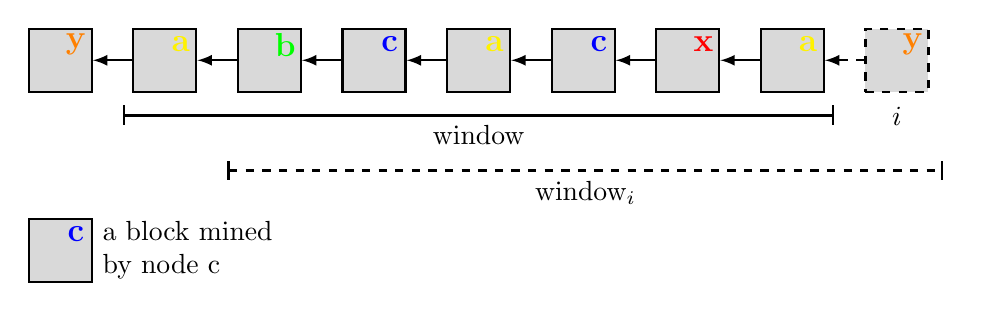
\begin{tikzpicture}
	[block/.style={rectangle,draw,thick, minimum size=.8cm, fill=gray!30!white},
	dblock/.style={block, dashed},
	noblock/.style={block, white},
	prev/.style={draw, -latex, thick}, 
	dprev/.style={prev, dashed},
	just/.style={-latex, double, thick, red},
	justarc/.style={out=135, in=45},
	interval/.style={|-|, dashed, thick},
	node distance =.5cm and .5cm]
	
	\node(b0)[block]{};
	\node(b1)[block, right=of b0]{};
	\draw[prev](b1) --node(x){} (b0);
	\node(b2)[block, right=of b1]{};
	\draw[prev](b2) --node(x1){} (b1);
	\node(b3)[block, right=of b2]{};
	\draw[prev](b3) -- (b2);
	\node(b4)[block, right=of b3]{};
	\draw[prev](b4) -- (b3);
	\node(b5)[block, right=of b4]{};
	\draw[prev](b5) -- (b4);
	\node(b6)[block, right=of b5]{};
	\draw[prev](b6) -- (b5);
	\node(b7)[block, right=of b6]{};
	\draw[prev](b7) -- (b6);
	\node(b8)[dblock, right=of b7]{};
	\draw[dprev](b8) -- node(y){} (b7);
	\node at ([yshift=-.3cm]b8.south){$i$};
	\node (y1) at ([xshift=.3cm]b8.east){};
	
	\node (Lb)[block] at ([yshift=-2cm]b0.south){};
	
	\begin{scope}[transform canvas={yshift =.2cm,xshift=.2cm}]
		\node at (b0)[orange]{\large\textbf{y}};
		\node at (b1)[yellow]{\large\textbf{a}};
		\node at (b2)[green]{\large\textbf{b}};
		\node at (b3)[blue]{\large\textbf{c}};
		\node at (b4)[yellow]{\large\textbf{a}};
		\node at (b5)[blue]{\large\textbf{c}};
		\node at (b6)[red]{\large\textbf{x}};
		\node at (b7)[yellow]{\large\textbf{a}};
		\node at (b8)[orange]{\large\textbf{y}};
		\node at (Lb)[blue]{\large\textbf{c}};
	\end{scope}
	
	
	\draw[transform canvas={yshift = -.7cm}, |-|,thick] (x) --node[below](w){window} (y);
	\node[below=of w]{};
	\draw[transform canvas={yshift = -1.4cm}, |-|,thick, dashed] (x1) --node[below](w){$\text{window}_i$} (y1);
	
	
	\node[right, align=left] at (Lb.east) {a block mined\\ by node c};
\end{tikzpicture}
	\caption{ByzCoin:An example for the Byzcoin sliding window. Nodes that have mined a block within the window get to sign the certificate for the new block ($i$) mined by y. Including $i$ we move to $\text{window}_i$}
	\label{fig:byzcoin}
\end{figure}

\begin{table}[h!]
	
	\centering
	\begin{tabular}{| r | c | c |}
		\hline
		node &  \parbox[t]{2.5cm}{voting power\\ in window\\} & \parbox[t]{2.5cm}{voting power\\ in $\text{window}_i$\\}\\
		\hline
		a & 3 & 2 \\ 
		b & 1 & 1 \\
		c & 2 & 2 \\
		x & 1 & 1 \\
		y & 0 & 1 \\
		\hline
	\end{tabular}
	\caption{Table showing voting power for Figure~\ref{fig:byzcoin}.}
\end{table}

\noindent
Note that when voting for block $i$ nodes a and c together hold $2/3$ of the voting power. This is no longer the case in $\text{window}_i$.
\end{example}

\pagebreak

\subsection{Casper FFG}
Casper FFG, requires nodes participating in the BFT protocol to deposit "Stake", i.e. Ether. A node depositing above a minimum of Ether may participate in the BFT protocol. Again, a node has a \emph{voting power} representing the fraction of the total "Stake".
Casper FFG uses Proof of Work to avoid the leader election problem. I.e. proposed blocks need to contain a proof of work. This limits the number of blocks that can be proposed concurrently.


\begin{example}
Figure~\ref{fig:casperFFG} shows an example of a blockchain using Casper-FFG. 
The committed blocks include transactions $t_1$ to $t_5$, where different stakeholders have deposited stake to obtain voting power. 
Note that:
\begin{itemize}
	\item Not every block must include a transaction depositing stake.
	\item One block could also include multiple transaction depositing stake.
	\item Stake is usually deposited for a fixed time, e.g. only for the confirmation of the next 100 blocks.
\end{itemize}
Table~\ref{tab:casper} shows the stake deposited, that is relevant for voting on the three batched blocks shown in Figure~\ref{fig:casperFFG}.
Note that $t_6$ is not included. That is because the block was not yet confirmed by the BFT algorithm.\\
\noindent
Table~\ref{tab:casper} shows that node a holds $\frac{2}{7}$ of the voting power. 

\begin{figure}[h!]
	%!TEX root = ../main.tex

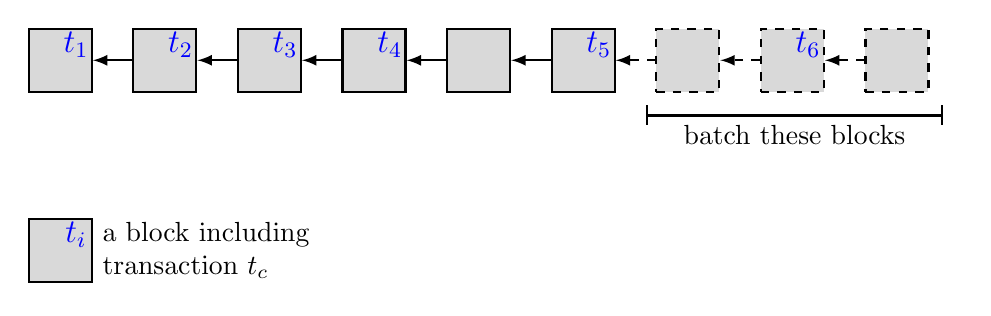
\begin{tikzpicture}
	[block/.style={rectangle,draw,thick, minimum size=.8cm, fill=gray!30!white},
	dblock/.style={block, dashed},
	noblock/.style={block, white},
	prev/.style={draw, -latex, thick}, 
	dprev/.style={prev, dashed},
	just/.style={-latex, double, thick, red},
	justarc/.style={out=135, in=45},
	interval/.style={|-|, dashed, thick},
	node distance =.5cm and .5cm]
	
	\node(b0)[block]{};
	\node(b1)[block, right=of b0]{};
	\draw[prev](b1) -- (b0);
	\node(b2)[block, right=of b1]{};
	\draw[prev](b2) --node(x1){} (b1);
	\node(b3)[block, right=of b2]{};
	\draw[prev](b3) -- (b2);
	\node(b4)[block, right=of b3]{};
	\draw[prev](b4) -- (b3);
	\node(b5)[block, right=of b4]{};
	\draw[prev](b5) -- (b4);
	\node(b6)[dblock, right=of b5]{};
	\draw[dprev](b6) --node(x){} (b5);
	\node(b7)[dblock, right=of b6]{};
	\draw[dprev](b7) -- (b6);
	\node(b8)[dblock, right=of b7]{};
	\draw[dprev](b8) -- node(y){} (b7);
	\node (y1) at ([xshift=.3cm]b8.east){};
	
	\node (Lb)[block] at ([yshift=-2cm]b0.south){};
	
	\begin{scope}[transform canvas={yshift =.2cm,xshift=.2cm}]
		\node at (b0)[blue]{\large\textbf{$t_1$}};
		\node at (b1)[blue]{\large\textbf{$t_2$}};
		\node at (b2)[blue]{\large\textbf{$t_3$}};
		\node at (b3)[blue]{\large\textbf{$t_4$}};
		% \node at (b4)[yellow]{\large\textbf{$t_5$}};
		\node at (b5)[blue]{\large\textbf{$t_5$}};
		% \node at (b6)[red]{\large\textbf{$t_7$}};
		\node at (b7)[blue]{\large\textbf{$t_6$}};
		% \node at (b8)[orange]{\large\textbf{$t_9$}};
		\node at (Lb)[blue]{\large\textbf{$t_i$}};
	\end{scope}
	
	
	\draw[transform canvas={yshift = -.7cm}, |-|,thick] (x) --node[below](w){batch these blocks} (y1);
	\node[below=of w]{};
	% \draw[transform canvas={yshift = -1.4cm}, |-|,thick, dashed] (x1) --node[below](w){$\text{window}_i$} (y1);
	
	
	\node[right, align=left] at (Lb.east) {a block including\\ transaction $t_c$};
\end{tikzpicture}
	\caption{A blockchain showing transactions that deposit stake.}
	\label{fig:casperFFG}
\end{figure}

\begin{table}[h!]
	
	\centering
	\begin{tabular}{| r | c | c |}
		\hline
		transaction & \parbox[t]{2.5cm}{deposited stake\\} & \parbox[t]{2.5cm}{submitted by}\\
		\hline
		$t_1$ & 2 eth & a \\ 
		$t_2$ & 2 eth & b \\
		$t_3$ & 1 eth & c \\
		$t_4$ & 1 eth & d \\
		$t_5$ & 1 eth & e \\
		\hline
		total & 7 eth &  \\
		\hline
		
	\end{tabular}
	\caption{Table showing voting power for Figure~\ref{fig:casperFFG}.}
	\label{tab:casper}
\end{table}	
\end{example}

\section{Algorand}

\href{https://dl.acm.org/doi/10.1145/3132747.3132757}{Algorand} is a hybrid blockchain that combines Proof of Stake with BFT.

Voting share is computed similar to Casper FFG.
The main difference is that Algorand does not rely on Proof of Work for leader election. Algorand uses Verifyable random functions for leader election. 
Below we present a simplified variant:

\begin{enumerate}
	\item Every block contains a $nonce$.
	\item To check if a node is leader for block $i$ he checks the following inequality:
	\[
		H(\text{Sign}_{pk}(nonce_{i-1}))< \text{stake}\cdot d
	\]
	Where $d$ is a fixed difficulty, stake is a factor, adjusting the difficulty based on a nodes stake or voting power. $\text{Sign}_{pk}(nonce_{i-1})$ is a signature of the previous nonce, with a nodes public key.
	\item If a node is a leader, he creates a new block, including 
	\[
		nonce_i = H(\text{Sign}_{pk}(nonce_{i-1}))
	\]
	\item Instead of waiting for just one proposed block, nodes wait for time $\Delta$ and several proposed blocks. They then sign the proposed block with the smallest $nonce$.
\end{enumerate}

To further improve scalability, Algorand uses the same mechanism used to select a leader, to select a committee, and requires only nodes in the committee to sign the certificate. 

\end{document}